\chapter{Results}
\label{ChapterResults}
This chapter analyzes the results of our experiments.


\section{Testbed Results}
\label{SectionTestbedResults}
We will divide our analysis as follows;
analysis for the results of the same classifier across different revealed percentages of data (chunks),
analysis for the results of different classifiers across the same revealed percentages of data (chunks)
and analysis for different classifiers and different percentages all together using the $F_{\beta}-measure$.
% could also be reorganized as results for testbed and results for recommender


% Models excluded due to performance
There were two classifiers that we excluded because they attained significantly inferior results compared to their published scores; these are KNNMSM and LS.
Specially on the InsectWingbeatSound data set, for which we attained a difference in performance of -45.71\% for KNNMSM and -20.71\% for LS than the results published by \cite{bagnall2017great}.


% Data sets that were not finished for remaining classifiers
For the remaining classifiers, not all of them were able to finish on all data sets within the time constraint.
Specially the multivariate archive, which was challenging for most of the algorithms in terms of memory and time complexity.
Our choice of adapting univariate classifiers for multivariate problems using column ensembling might have made things even more challenging;
because this technique fits for each dimension in the data sets a classifier, which is a memory and space extensive solution.
This was clearly evident for the runs as the number of dimensions of the data sets increased.

TSF was the most successful algorithm in finishing the biggest number of datasets. It was able to finish all the data sets from both archives, with the exception of FaceDetection only.
WEASEL was the second best, finishing all data sets from both archives, except for the largest three multivariate data sets; DuckDuckGeese, FaceDetection and PEMS-SF.
WEASEL is known for its quality and speed but not for scalability \cite{lucas2019proximity}, it failed these data sets due to out of memory errors.
CBoss failed to run on DuckDuckGeese, FaceDetection, PEMS-SF and MotorImagery within our time constraint.
ST is known to be one of the slowest algorithms, but we use an enhanced version to accelerate its performance. However, ST was not able to finish within our time limit on 15 multivariate datasets; due to its linear time complexity with the number of dimensions. It hit the limit of the time constraint once the number dimensions reached 6.
%ERing,BasicMotions,Cricket,LSST,RacketSports,SelfRegulationSCP1,SelfRegulationSCP2,HandMovementDirection,NATOPS
%FingerMovements,Heartbeat,MotorImagery,FaceDetection,PEMS-SF,DuckDuckGeese
It has also failed on the Fungi dataset, because it couldn't find high quality shapelets during the contract time that we cofigured it to use.
The slowest of all and which achieved the least progress on the data sets was PForest. It finished a total of 7 multivariate data Sets and 35 univariate data sets.
Although PForest can attain quasi linear training times with the size of training data, but it has a training complexity, which can be quadratic with length based on its randomly selected distance measure.
This is why PForest hit the time contraint easily as the length of the time series increased.
All 5 classifiers completed 36 common data sets. TSF, WEASEL and CBoss finished more than 72 data sets, ST finished 61 data sets and PForest finished 42 data sets.

Tables \ref{tab:longresults} and \ref{tab:longresults_1} present the results of our experiments for the used 5 classifiers on all 77 data sets.
We display values for balanced accuracy, $F_{\beta}-measure$ value and revealed\% for each classifier.
The default train/test split of the data sets was used for all data runs.

\begin{landscape}
    \begin{longtable}{|l|llll|llll|llll|}
      \caption{$F_{\beta}$ scores for CBoss, PForest and ST on 77 data sets for all chunks}\\
      \hline
      \multirow{2}{*}{\textbf{Data set}} & 
      \multicolumn{4}{c}{\textbf{CBoss}} & \multicolumn{4}{c}{\textbf{PForest}} & \multicolumn{4}{c}{\textbf{ST}} \\
      & \textbf{10\%} & \textbf{20\%} & \textbf{30\%} & \textbf{100\%} & \textbf{10\%} & \textbf{20\%} & \textbf{30\%} & \textbf{100\%} & \textbf{10\%} & \textbf{20\%} & \textbf{30\%} & \textbf{100\%} \\ [0.5ex]
      \hline
      \endfirsthead % <-- This denotes the end of the header, which will be shown on the first page only
      \caption{$F_{\beta}$ scores for CBoss, PForest and ST on 77 data sets for all chunks (continued)}\\
      \hline
      \multirow{2}{*}{\textbf{Data set}} & 
      \multicolumn{4}{c}{\textbf{CBoss}} & \multicolumn{4}{c}{\textbf{PForest}} & \multicolumn{4}{c}{\textbf{ST}} \\
      & \textbf{10\%} & \textbf{20\%} & \textbf{30\%} & \textbf{100\%} & \textbf{10\%} & \textbf{20\%} & \textbf{30\%} & \textbf{100\%} & \textbf{10\%} & \textbf{20\%} & \textbf{30\%} & \textbf{100\%} \\ [0.5ex]
      \hline
      \endhead % <-- Everything between \endfirsthead and \endhead will be shown as a header on every page
      ACSF1 & 77.78 & 74.77 & 70.81 & 87.80 & 65.27 & 48.19 & 37.80 &   & 80.30 & 81.63 & 84.33 & 78.47 \\ \hline
      AtrialFibrillation & 66.67 & 48.00 & 43.10 & 16.67 & 70.00 & 60.00 & 40.00 & 28.57 & 71.43 & 48.00 & 53.85 & 34.78 \\ \hline
      BasicMotions & 71.05 & 84.21 & 100.00 & 100.00 & 67.39 & 61.54 & 55.88 & 70.59 &   &   &   &   \\ \hline
      Beef & 67.65 & 50.00 & 58.00 & 76.19 & 67.14 & 51.06 & 37.10 & 25.53 & 66.67 & 55.81 & 53.85 & 76.19 \\ \hline
      Car & 68.46 & 53.93 & 51.89 & 80.00 & 71.43 & 53.33 & 44.74 & 42.80 & 68.75 & 59.26 & 61.34 & 78.09 \\ \hline
      Chinatown & 63.88 & 65.26 & 71.10 & 93.88 & 65.48 & 54.84 & 97.48 & 96.74 & 66.30 & 73.11 & 72.93 & 96.38 \\ \hline
      CinCECGTorso & 68.54 & 54.33 & 45.28 & 75.78 &   &   &   &   & 67.52 & 55.62 & 56.06 & 89.88 \\ \hline
      Coffee & 73.14 & 95.73 & 95.66 & 100.00 & 76.42 & 65.12 & 71.15 & 100.00 & 79.17 & 84.85 & 95.66 & 91.23 \\ \hline
      Computers & 77.17 & 71.68 & 68.11 & 64.25 & 74.27 & 62.89 & 57.14 & 55.37 & 75.25 & 67.80 & 66.28 & 63.82 \\ \hline
      Cricket & 65.69 & 74.23 & 81.71 & 100.00 &   &   &   &   &   &   &   &   \\ \hline
      Earthquakes & 80.68 & 76.06 & 73.98 & 70.39 & 80.68 & 76.06 & 73.98 & 71.19 & 75.36 & 76.06 & 73.98 & 59.50 \\ \hline
      ECG200 & 69.42 & 56.74 & 47.78 & 79.62 & 76.67 & 77.67 & 54.83 & 87.80 & 76.32 & 80.81 & 75.75 & 83.09 \\ \hline
      ECG5000 & 69.12 & 67.39 & 81.34 & 92.83 & 74.69 & 65.85 & 61.37 & 55.33 & 81.47 & 87.15 & 89.73 & 92.48 \\ \hline
      ECGFiveDays & 74.41 & 61.68 & 56.06 & 100.00 & 72.86 & 65.43 & 60.06 & 82.08 & 72.29 & 67.34 & 65.21 & 99.85 \\ \hline
      ElectricDevices & 70.24 & 57.31 & 55.78 & 65.58 &   &   &   &   & 69.61 & 55.75 & 43.04 & 32.92 \\ \hline
      EOGHorizontalSignal & 65.06 & 46.82 & 40.58 & 42.00 & 65.09 & 46.14 & 33.93 &   & 65.22 & 46.59 & 40.58 & 41.73 \\ \hline
      EOGVerticalSignal & 65.38 & 47.04 & 37.77 & 36.93 &   &   &   &   & 65.06 & 46.74 & 40.95 & 33.53 \\ \hline
      Epilepsy & 96.62 & 100.00 & 100.00 & 100.00 &   &   &   &   & 79.93 & 79.20 & 86.78 & 98.19 \\ \hline
      ERing & 68.00 & 53.40 & 51.35 & 87.36 & 66.17 & 50.15 & 40.61 & 45.18 &   &   &   &   \\ \hline
      EthanolConcentration & 67.41 & 51.27 & 42.35 & 35.79 &   &   &   &   & 69.54 & 55.90 & 47.29 & 55.41 \\ \hline
      EthanolLevel & 67.79 & 51.81 & 43.46 & 39.37 &   &   &   &   & 68.66 & 56.18 & 47.19 & 30.85 \\ \hline
      FingerMovements & 71.05 & 62.02 & 55.26 & 51.47 &   &   &   &   &   &   &   &   \\ \hline
      FordA & 80.03 & 83.41 & 82.37 & 68.33 &   &   &   &   & 70.87 & 61.50 & 59.44 & 49.67 \\ \hline
      FordB & 77.65 & 74.65 & 72.32 & 56.72 &   &   &   &   & 72.85 & 60.17 & 60.37 & 48.13 \\ \hline
      FreezerRegularTrain & 72.22 & 97.15 & 99.87 & 99.56 & 78.90 & 62.50 & 89.63 & 90.49 & 72.37 & 94.33 & 99.87 & 99.87 \\ \hline
      FreezerSmallTrain & 72.26 & 94.57 & 99.74 & 96.56 & 75.18 & 63.60 & 72.00 & 66.11 & 71.91 & 91.27 & 99.82 & 99.96 \\ \hline
      Fungi & 65.16 & 45.53 & 33.24 &   & 64.92 & 47.57 & 43.73 & 89.47 &   &   &   &   \\ \hline
      Ham & 71.88 & 61.31 & 55.00 & 61.54 & 72.11 & 62.69 & 55.59 & 65.63 & 71.88 & 60.87 & 58.00 & 71.91 \\ \hline
      HandMovementDirection & 68.14 & 50.08 & 43.28 & 31.49 & 66.70 & 51.84 & 47.37 & 32.75 &   &   &   &   \\ \hline
      Handwriting & 64.69 & 44.49 & 37.53 & 41.10 &   &   &   &   & 64.69 & 44.65 & 35.96 & 31.14 \\ \hline
      HouseTwenty & 71.72 & 78.55 & 84.89 & 96.87 & 81.90 & 75.44 & 71.84 & 87.70 & 76.27 & 77.91 & 82.39 & 80.81 \\ \hline
      InsectEPGRegularTrain & 96.72 & 94.32 & 100.00 & 100.00 & 100.00 & 99.50 & 100.00 & 100.00 & 69.18 & 55.92 & 48.55 & 98.50 \\ \hline
      InsectEPGSmallTrain & 91.29 & 100.00 & 94.67 & 100.00 & 99.50 & 90.05 & 98.51 & 100.00 & 69.18 & 55.77 & 48.33 & 96.51 \\ \hline
      InsectWingbeatSound & 65.22 & 48.98 & 45.17 & 49.64 &   &   &   &   & 65.21 & 48.51 & 39.14 & 56.54 \\ \hline
      ItalyPowerDemand & 69.43 & 57.66 & 78.91 & 86.41 & 70.71 & 71.06 & 58.02 & 94.95 & 68.66 & 58.52 & 69.13 & 94.47 \\ \hline
      LargeKitchenAppliances & 72.73 & 61.86 & 57.14 & 72.89 & 69.79 & 56.07 & 50.45 & 37.83 & 69.04 & 54.95 & 47.26 & 61.54 \\ \hline
      Libras & 62.41 & 44.04 & 41.36 & 79.36 & 62.69 & 42.74 & 32.38 & 5.41 & 62.99 & 45.24 & 39.66 & 83.87 \\ \hline
      Lightning2 & 73.28 & 64.38 & 58.50 & 69.23 & 70.89 & 66.12 & 58.50 & 80.31 & 73.28 & 59.66 & 55.37 & 65.65 \\ \hline
      Lightning7 & 69.41 & 55.41 & 52.18 & 69.45 & 66.19 & 49.74 & 39.63 & 25.66 & 65.84 & 47.71 & 42.80 & 64.97 \\ \hline
      LSST & 62.41 & 51.74 & 45.33 & 45.29 &   &   &   &   &   &   &   &   \\ \hline
      Meat & 86.36 & 70.59 & 85.00 & 85.83 & 73.53 & 57.14 & 46.43 & 59.77 & 80.77 & 92.31 & 80.12 & 95.87 \\ \hline
      MoteStrain & 71.39 & 74.58 & 63.24 & 93.20 & 70.60 & 78.17 & 76.93 & 86.88 & 73.41 & 59.66 & 71.72 & 89.92 \\ \hline
      NATOPS & 64.69 & 51.86 & 46.40 & 80.00 & 63.76 & 47.53 & 37.95 & 18.60 &   &   &   &   \\ \hline
      NonInvasiveFetalECGThorax1 & 71.16 & 56.47 & 63.73 & 78.51 &   &   &   &   & 72.98 & 70.56 & 62.04 & 28.48 \\ \hline
      NonInvasiveFetalECGThorax2 & 68.38 & 70.68 & 57.54 & 82.27 &   &   &   &   & 67.95 & 74.08 & 75.43 & 51.36 \\ \hline
      OliveOil & 69.35 & 85.71 & 92.11 & 83.87 & 66.67 & 50.00 & 50.00 & 51.13 & 77.27 & 92.31 & 88.46 & 87.80 \\ \hline
      Phoneme & 66.27 & 50.61 & 42.38 & 26.83 & 64.43 & 44.79 & 32.33 & 1.35 & 66.47 & 50.18 & 41.30 & 23.45 \\ \hline
      PigAirwayPressure & 66.05 & 50.82 & 41.85 & 91.15 &   &   &   &   & 65.81 & 50.06 & 51.30 & 75.43 \\ \hline
      PigArtPressure & 97.71 & 99.40 & 98.22 & 97.61 &   &   &   &   & 88.81 & 90.73 & 95.34 & 95.24 \\ \hline
      PigCVP & 80.77 & 87.86 & 92.57 & 94.06 & 64.43 & 45.29 &   &   & 68.81 & 58.92 & 72.51 & 72.19 \\ \hline
      Plane & 67.21 & 48.84 & 52.23 & 100.00 & 69.09 & 53.16 & 56.37 & 100.00 & 67.36 & 63.16 & 63.57 & 100.00 \\ \hline
      PowerCons & 74.32 & 71.64 & 75.95 & 90.46 & 76.47 & 67.92 & 68.47 & 99.31 & 73.68 & 61.80 & 66.73 & 92.48 \\ \hline
      RacketSports & 67.49 & 50.96 & 43.89 & 77.24 & 69.14 & 53.19 & 46.54 & 38.04 &   &   &   &   \\ \hline
      RefrigerationDevices & 72.80 & 60.00 & 56.47 & 48.83 & 70.00 & 58.48 & 55.30 & 40.66 & 72.46 & 60.36 & 57.14 & 50.45 \\ \hline
      Rock & 70.83 & 58.82 & 61.11 & 87.80 & 68.18 & 53.33 & 42.78 & 40.53 & 67.54 & 51.28 & 44.74 & 85.44 \\ \hline
      ScreenType & 70.16 & 58.59 & 52.12 & 43.79 & 69.33 & 54.05 &   &   & 69.08 & 56.82 & 50.45 & 43.00 \\ \hline
      SelfRegulationSCP1 & 76.14 & 70.52 & 68.62 & 74.49 &   &   &   &   &   &   &   &   \\ \hline
      SelfRegulationSCP2 & 72.09 & 64.00 & 62.11 & 47.20 & 70.81 &   &   &   &   &   &   &   \\ \hline
      SemgHandGenderCh2 & 78.10 & 69.57 & 76.02 & 85.63 &   &   &   &   & 69.11 & 70.90 & 82.35 & 77.52 \\ \hline
      SemgHandMovementCh2 & 66.33 & 48.98 & 39.21 & 59.18 &   &   &   &   & 66.89 & 55.73 & 47.47 & 41.83 \\ \hline
      SemgHandSubjectCh2 & 67.89 & 51.65 & 49.14 & 70.96 &   &   &   &   & 68.37 & 62.18 & 61.72 & 52.72 \\ \hline
      SmallKitchenAppliances & 79.64 & 73.53 & 68.42 & 73.78 & 69.38 & 58.37 & 48.54 &   & 71.13 & 55.35 & 53.21 & 74.08 \\ \hline
      SonyAIBORobotSurface1 & 72.28 & 80.16 & 52.72 & 41.26 & 81.68 & 83.07 & 84.85 & 79.08 & 70.60 & 71.04 & 70.17 & 92.02 \\ \hline
      SonyAIBORobotSurface2 & 70.00 & 66.69 & 85.02 & 89.47 & 75.47 & 66.44 & 73.24 & 85.48 & 75.54 & 67.12 & 64.01 & 89.47 \\ \hline
      StandWalkJump & 70.00 & 50.00 & 46.43 & 28.57 & 68.75 & 52.17 & 46.43 &   & 68.75 & 57.14 & 46.43 & 28.57 \\ \hline
      StarlightCurves & 68.05 & 52.71 & 45.23 & 96.88 &   &   &   &   & 74.31 & 69.86 & 79.00 & 91.51 \\ \hline
      Strawberry & 76.43 & 69.16 & 95.73 & 96.98 & 76.43 & 69.16 & 65.63 & 90.39 & 80.33 & 77.69 & 76.86 & 92.68 \\ \hline
      Trace & 68.35 & 57.55 & 70.00 & 100.00 & 72.73 & 61.54 & 54.65 & 47.43 & 68.18 & 50.63 & 39.55 & 100.00 \\ \hline
      TwoLeadECG & 72.36 & 60.84 & 65.52 & 99.56 & 75.81 & 70.10 & 67.14 & 93.07 & 72.23 & 61.76 & 63.57 & 99.78 \\ \hline
      UWaveGestureLibrary & 65.46 & 48.39 & 39.30 & 81.57 &   &   &   &   & 65.69 & 47.76 & 36.88 & 85.95 \\ \hline
      Wafer & 92.71 & 98.07 & 98.47 & 99.61 & 93.19 & 95.00 & 89.55 & 99.35 & 94.50 & 100.00 & 99.49 & 100.00 \\ \hline
      Wine & 75.96 & 63.34 & 71.80 & 69.57 & 71.77 & 64.29 & 70.30 & 53.78 & 74.77 & 65.26 & 65.99 & 71.62 \\ \hline
    \label{tab:longresults}
    \end{longtable}
\end{landscape}

\begin{landscape}
  \begin{longtable}{|l|llll|llll|}
    \caption{$F_{\beta}$ scores for TSF and WEASEL on 77 data sets for all chunks}\\
    \hline
    \multirow{2}{*}{\textbf{Data set}} & 
    \multicolumn{4}{c}{\textbf{TSF}} & \multicolumn{4}{c}{\textbf{WEASEL}} \\
    & \textbf{10\%} & \textbf{20\%} & \textbf{30\%} & \textbf{100\%} & \textbf{10\%} & \textbf{20\%} & \textbf{30\%} & \textbf{100\%} \\ [0.5ex]
    \hline
    \endfirsthead % <-- This denotes the end of the header, which will be shown on the first page only
    \caption{$F_{\beta}$ scores for TSF and WEASEL on 77 data sets for all chunks (continued)}\\
    \hline
    \multirow{2}{*}{\textbf{Data set}} & 
    \multicolumn{4}{c}{\textbf{TSF}} & \multicolumn{4}{c}{\textbf{WEASEL}} \\
    & \textbf{10\%} & \textbf{20\%} & \textbf{30\%} & \textbf{100\%} & \textbf{10\%} & \textbf{20\%} & \textbf{30\%} & \textbf{100\%} \\ [0.5ex]
    \hline
    \endhead % <-- Everything between \endfirsthead and \endhead will be shown as a header on every page
    ACSF1 & 77.40 & 68.38 & 66.13 & 59.77 & 78.99 & 76.19 & 68.42 & 89.00 \\ \hline
    AtrialFibrillation & 66.67 & 54.55 & 34.38 & 22.54 & 71.43 & 54.55 & 43.10 & 22.54 \\ \hline
    BasicMotions & 82.00 & 96.97 & 100.00 & 100.00 & 75.00 & 100.00 & 100.00 & 100.00 \\ \hline
    Beef & 78.57 & 72.73 & 72.73 & 65.12 & 65.79 & 51.06 & 50.00 & 76.19 \\ \hline
    Car & 75.00 & 71.64 & 66.13 & 66.93 & 68.46 & 53.93 & 45.58 & 83.87 \\ \hline
    Chinatown & 95.61 & 98.20 & 97.84 & 95.66 & 63.88 & 47.42 & 39.12 & 93.53 \\ \hline
    CinCECGTorso & 72.35 & 67.48 & 73.58 & 88.76 & 76.16 & 81.60 & 68.91 & 95.16 \\ \hline
    Coffee & 89.44 & 84.85 & 80.57 & 100.00 & 73.14 & 91.80 & 65.60 & 100.00 \\ \hline
    Computers & 78.41 & 72.99 & 70.97 & 66.42 & 71.93 & 70.42 & 70.32 & 67.29 \\ \hline
    Cricket & 84.45 & 85.21 & 91.79 & 89.80 & 71.56 & 65.75 & 77.81 & 98.27 \\ \hline
    Earthquakes & 80.68 & 76.06 & 73.98 & 70.39 & 80.68 & 75.54 & 73.37 & 70.39 \\ \hline
    ECG200 & 84.48 & 85.11 & 86.32 & 81.93 & 74.39 & 59.26 & 51.19 & 81.93 \\ \hline
    ECG5000 & 92.19 & 91.23 & 90.26 & 92.18 & 74.10 & 80.70 & 74.52 & 92.64 \\ \hline
    ECGFiveDays & 75.16 & 67.28 & 62.13 & 90.32 & 73.20 & 63.15 & 58.82 & 99.85 \\ \hline
    ElectricDevices & 73.15 & 63.54 & 61.22 & 63.55 & 75.13 & 66.37 & 60.86 & 72.62 \\ \hline
    EOGHorizontalSignal & 65.44 & 46.59 & 39.58 & 45.81 & 64.96 & 47.43 & 36.72 & 42.27 \\ \hline
    EOGVerticalSignal & 65.25 & 46.82 & 40.45 & 39.85 & 64.90 & 46.74 & 35.13 & 27.14 \\ \hline
    Epilepsy & 91.69 & 97.35 & 97.33 & 96.40 & 98.25 & 100.00 & 100.00 & 100.00 \\ \hline
    ERing & 75.47 & 76.89 & 82.66 & 94.05 & 68.56 & 58.20 & 58.76 & 94.05 \\ \hline
    EthanolConcentration & 70.45 & 58.38 & 49.96 & 36.88 & 67.70 & 51.77 & 46.49 & 50.73 \\ \hline
    EthanolLevel & 69.42 & 54.64 & 45.54 & 39.37 & 67.42 & 51.68 & 42.40 & 43.85 \\ \hline
    FingerMovements & 70.62 & 62.50 & 55.88 & 44.44 & 72.47 & 62.02 & 55.88 & 53.51 \\ \hline
    FordA & 79.40 & 75.70 & 75.85 & 77.74 & 83.29 & 79.70 & 91.60 & 95.77 \\ \hline
    FordB & 74.88 & 67.22 & 64.00 & 63.52 & 76.30 & 76.96 & 64.17 & 78.30 \\ \hline
    FreezerRegularTrain & 96.45 & 99.82 & 99.82 & 98.91 & 72.22 & 92.87 & 73.29 & 97.51 \\ \hline
    FreezerSmallTrain & 88.93 & 97.98 & 99.78 & 80.85 & 72.22 & 89.55 & 64.56 & 95.05 \\ \hline
    Fungi & 65.54 & 52.80 & 54.89 & 93.37 & 64.86 & 45.95 & 34.29 & 94.68 \\ \hline
    Ham & 74.71 & 76.36 & 72.73 & 74.04 & 72.58 & 62.22 & 55.00 & 59.52 \\ \hline
    HandMovementDirection & 67.70 & 54.21 & 43.94 & 49.85 & 67.29 & 50.08 & 38.92 & 31.49 \\ \hline
    Handwriting & 65.70 & 49.52 & 43.41 & 26.49 & 64.71 & 44.16 & 33.38 & 26.39 \\ \hline
    HouseTwenty & 86.28 & 92.25 & 89.27 & 77.91 & 88.64 & 94.07 & 92.04 & 95.83 \\ \hline
    InsectEPGRegularTrain & 100.00 & 100.00 & 100.00 & 100.00 & 100.00 & 100.00 & 100.00 & 100.00 \\ \hline
    InsectEPGSmallTrain & 100.00 & 100.00 & 100.00 & 100.00 & 100.00 & 100.00 & 100.00 & 100.00 \\ \hline
    InsectWingbeatSound & 71.15 & 64.89 & 63.83 & 56.33 & 65.66 & 53.33 & 48.13 & 58.39 \\ \hline
    ItalyPowerDemand & 75.92 & 71.42 & 76.09 & 95.31 & 69.43 & 58.41 & 55.66 & 91.17 \\ \hline
    LargeKitchenAppliances & 72.12 & 60.61 & 54.17 & 51.54 & 68.16 & 54.05 & 46.29 & 63.82 \\ \hline
    Libras & 67.90 & 64.65 & 68.53 & 76.82 & 63.52 & 48.98 & 50.78 & 83.87 \\ \hline
    Lightning2 & 73.28 & 68.93 & 70.39 & 65.65 & 73.28 & 66.12 & 64.14 & 62.12 \\ \hline
    Lightning7 & 67.55 & 61.86 & 58.96 & 69.45 & 68.67 & 52.42 & 41.50 & 67.95 \\ \hline
    LSST & 68.85 & 57.77 & 52.68 & 44.89 & 68.23 & 58.44 & 51.08 & 53.18 \\ \hline
    Meat & 83.33 & 82.76 & 83.33 & 91.80 & 76.09 & 61.54 & 46.43 & 81.93 \\ \hline
    MoteStrain & 87.89 & 86.66 & 86.98 & 84.52 & 77.16 & 78.17 & 79.46 & 94.18 \\ \hline
    NATOPS & 64.43 & 52.07 & 51.71 & 76.82 & 64.26 & 52.69 & 54.07 & 80.00 \\ \hline
    NonInvasiveFetalECGThorax1 & 83.62 & 79.59 & 78.29 & 84.53 & 64.54 & 49.42 & 40.60 &   \\ \hline
    NonInvasiveFetalECGThorax2 & 86.97 & 83.53 & 80.52 & 87.84 & 64.53 & 46.37 & 36.14 & 90.45 \\ \hline
    OliveOil & 80.00 & 80.00 & 88.46 & 83.87 & 65.79 & 48.98 & 44.74 & 87.80 \\ \hline
    Phoneme & 65.76 & 49.36 & 39.78 & 16.52 & 66.84 & 51.35 & 43.60 & 25.78 \\ \hline
    PigAirwayPressure & 65.34 & 47.22 & 35.17 & 18.51 & 68.07 & 57.30 & 49.68 & 58.65 \\ \hline
    PigArtPressure & 66.24 & 50.67 & 43.69 & 35.15 & 93.70 & 96.52 & 95.91 & 100.00 \\ \hline
    PigCVP & 65.99 & 49.03 & 38.80 & 23.63 & 71.42 & 68.09 & 81.55 & 91.73 \\ \hline
    Plane & 91.18 & 97.67 & 95.38 & 98.81 & 66.15 & 48.84 & 86.92 & 100.00 \\ \hline
    PowerCons & 81.03 & 77.42 & 77.96 & 99.31 & 73.23 & 64.57 & 62.59 & 95.19 \\ \hline
    RacketSports & 75.17 & 72.55 & 78.21 & 87.96 & 69.14 & 55.88 & 52.32 & 84.85 \\ \hline
    RefrigerationDevices & 72.94 & 63.29 & 58.00 & 53.17 & 69.69 & 57.92 & 52.90 & 44.84 \\ \hline
    Rock & 71.74 & 64.52 & 63.92 & 69.48 & 67.24 & 57.97 & 39.11 & 76.19 \\ \hline
    ScreenType & 69.89 & 57.80 & 52.58 & 38.08 & 71.01 & 57.58 & 52.27 & 47.76 \\ \hline
    SelfRegulationSCP1 & 80.97 & 83.89 & 82.65 & 76.04 & 76.73 & 86.37 & 78.45 & 76.04 \\ \hline
    SelfRegulationSCP2 & 72.93 & 63.16 & 58.36 & 42.26 & 72.09 & 63.16 & 61.72 & 55.12 \\ \hline
    SemgHandGenderCh2 & 81.50 & 89.05 & 87.58 & 91.20 & 76.67 & 70.07 & 66.25 & 74.87 \\ \hline
    SemgHandMovementCh2 & 73.56 & 67.92 & 71.26 & 81.28 & 66.33 & 48.98 & 39.60 & 25.13 \\ \hline
    SemgHandSubjectCh2 & 75.86 & 78.26 & 76.96 & 89.40 & 66.67 & 50.00 & 45.29 & 58.72 \\ \hline
    SmallKitchenAppliances & 77.27 & 70.59 & 66.38 & 79.54 & 74.35 & 70.26 & 58.70 & 67.29 \\ \hline
    SonyAIBORobotSurface1 & 78.73 & 77.20 & 74.60 & 64.45 & 72.12 & 88.41 & 86.21 & 80.03 \\ \hline
    SonyAIBORobotSurface2 & 80.88 & 79.26 & 77.85 & 74.13 & 79.73 & 77.04 & 89.81 & 93.40 \\ \hline
    StandWalkJump & 71.43 & 54.55 & 53.85 & 34.78 & 71.43 & 57.14 & 58.00 & 28.57 \\ \hline
    StarlightCurves & 92.50 & 94.13 & 95.21 & 95.28 & 69.11 & 52.94 & 43.76 & 93.75 \\ \hline
    Strawberry & 89.57 & 90.24 & 94.78 & 93.66 & 76.43 & 69.16 & 65.63 & 95.65 \\ \hline
    Trace & 77.40 & 73.39 & 68.42 & 98.75 & 67.24 & 54.42 & 50.00 & 100.00 \\ \hline
    TwoLeadECG & 80.11 & 82.76 & 93.48 & 70.18 & 72.23 & 62.30 & 64.93 & 99.78 \\ \hline
    UWaveGestureLibrary & 70.06 & 67.72 & 71.01 & 81.93 & 65.24 & 49.71 & 42.90 & 77.61 \\ \hline
    Wafer & 99.48 & 99.06 & 99.31 & 99.31 & 99.32 & 88.10 & 87.63 & 99.96 \\ \hline
    Wine & 77.27 & 66.26 & 61.98 & 67.53 & 72.22 & 61.54 & 60.71 & 75.77 \\ \hline
  \label{tab:longresults_1}
  \end{longtable}
\end{landscape}

We divide our analysis into three parts: a comparison of the effect of data chopping within the same classifier,
comparison on the effect of data chopping across different classifiers and unified comparison between all classifiers
across all data chops.
Since some of the analysis results we present include comparisons between the same classifier trained on different percentages of data, we use a special naming convention.
We name the classifiers using the format $NameOfClassifier\_Revealed\%$, where the first part of the name refer to the name of the classifier
and the second part refers to the percentage of data used to train the classifier. For example, $TSF\_10$ refers to classifier TSF which was trained on 10\% of the data length.
This naming convention helps clarify the type of the classifier and the context of comparison regardless of the type of analysis being discussed.


\subsection{Results Across Classifiers}
\label{SubsectionAcrossComparison}
An aspect to investigate within the early classification context is the relative performance of classifiers to each other while more data becomes available to train on.
We fix the percentage of data revealed, revealed\%, and compare the performance of classifiers, which is represented by their ranking based on the value of $F_{\beta}-measure$.
We will dig deeper into the properties of the data sets, to explore the relation between the characteristics of the data and the best performing algorithm.

To better understand the actual performance of the classifiers on the data sets and assess the quality of their results, we introduce a new baseline classifier to the comparison.
The baseline classifier always predicts the majority class of a given data set.
We name the classifier \emph{dummy}; as an indication of its role in the comparisons.
To ensure the integrity of our comparisons, we calculate balanced accuracy and $F_{\beta}-measure$ for the dummy classifier on all data sets and for the same 4 chunks.
Although the dummy classifier will always predict the majority class and thus score the same balanced accuracy, but its $F_{\beta}-measure$ will differ based on the revealed\%.

Figure \ref{fig:CDAcross} shows the critical difference diagram across all the classifiers and for a fixed revealed percentage of data.
In the beginning when only 10\% of the data is revevaled, TSF is significantly better than all the other classifiers.
The remaining four classifiers form a clique together and are not significantly different from the dummy classifier.
Inside that clique, CBoss is the best classifier, WEASEL is the second best and both PForest and ST are almost identical in their ranking.

\begin{figure} [!htb]
  \centering
  \begin{tabular}{ccc}
  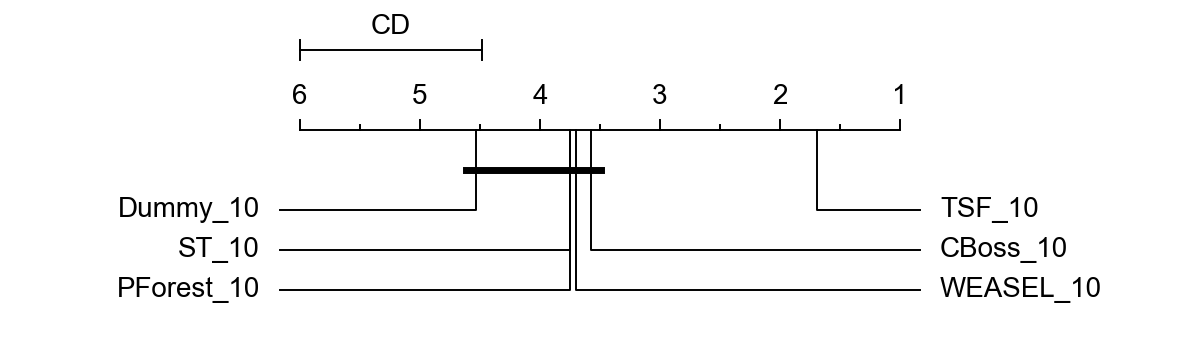
\includegraphics[width=0.49\textwidth]{cd_f_score_across_10pct_with_dummy.png} & & 
  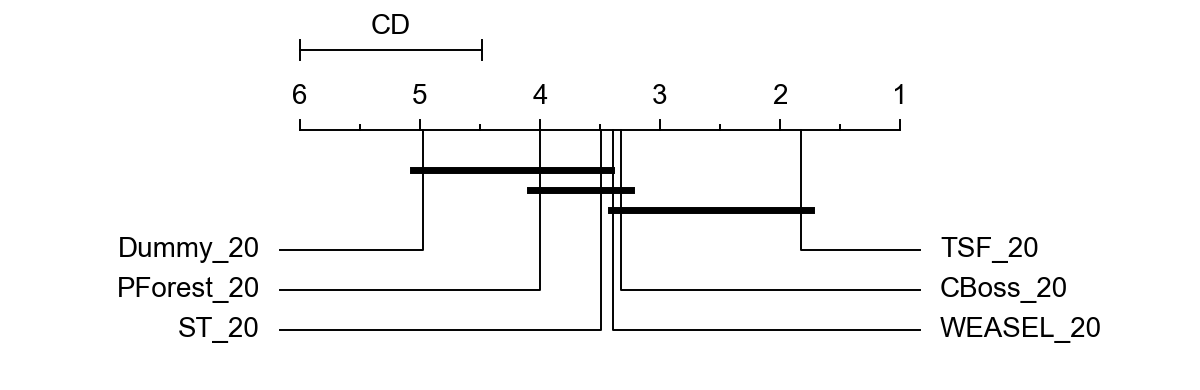
\includegraphics[width=0.49\textwidth]{cd_f_score_across_20pct_with_dummy.png} \\
  \textbf{(a) 10\% chunk} & & \textbf{(b) 20\% chunk} \\[6pt]
  \end{tabular}
  \begin{tabular}{ccc}
  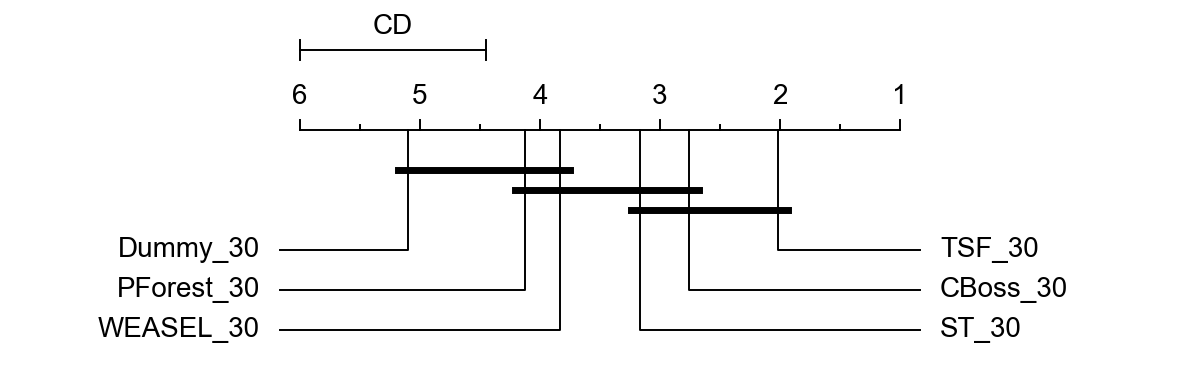
\includegraphics[width=0.49\textwidth]{cd_f_score_across_30pct_with_dummy.png} & & 
  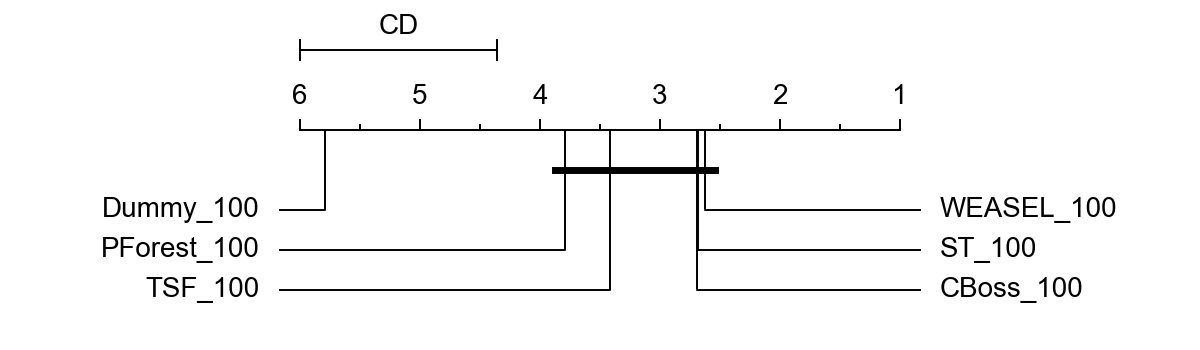
\includegraphics[width=0.49\textwidth]{cd_f_score_across_100pct_with_dummy.png} \\
  \textbf{(c) 30\% chunk} & & \textbf{(d) 100\% chunk}  \\[6pt]
  \end{tabular}
  \caption{Critical Difference diagrams per chunk across all classifiers}
  \label{fig:CDAcross}
\end{figure}

When the revealed percentage is increased to 20\%, TSF still prevails as the first classifier but with no significant different to CBoss and WEASEL.
There is still no significant difference between the PForest, ST and WEASEL and between the dummy classifier.
ST is able to learn better shapelets on the data and beats PForest.
On the third chunk, CBoss and ST are not significantly different from TSF and join it to form the first clique.
While WEASEL and PForest are not significantly different from the dummy classifier.
The middle clique shows no significant difference between CBoss, ST, WEASEL and PForest. However WEASEL and PForest are both significantly worse than TSF.
On the full length of data, the 5 classifiers are all not significantly different from each other.
WEASEL attains the best ranking followed by ST and CBoss which are identical, while TSF loses its edge on full length data.
PForest ranks the last among the 5 classifiers. All the classifiers form one clique which is significantly better than the dummy classifier.

The most apparent conclusion from the graphs is that TSF is able to do better on data sets during the earlier stages of the early classification context.
We believe the reason why TSF is always better on the shorter chunks of data; is because it uses three simple aggregations as features and doesn't depend on advanced features like the other classifiers do.
On the other side, the BOP technique applied by WEASEL and CBoss is challenged by the chopping, which notably decreases the chances of repetition of distinctive patterns in the data within such a small length.
PForest is also expected to perform badly as it needs to stretch the extent of its elastic distance measures; by measuring distances between testing instances which are 10 times the length of the training instances.
ST gets the lowest scores because in cases like our experiments where majority of the data is chopped, it is very hard to find shapelets that can uniquely indentify the different classes by learning on only the first 10\% of the data.
An obvious change is visible when more data is made available for training, the techniques of; WEASEL; CBoss and ST are able to make use of the more available information
to find better and more distinctive features in the data; which helps them be more competent.
Also PForest is able to score get better performances; because its elastic distance measure do not have to compensate for the big difference in length.


\subsection{Data Set characteristics and performance in early classification context}
\label{SubsectionDataCharacteristicsandPerformance}
The goal of our reasearch is to learn a recommender which can suggest the best classifiers to unseen data sets.
The recommender analyzes the characteristics of the data set and then based on the performance from previous experiments, it suggests the most suitable classifiers.
Thus it could be very convenient if the characteristics of the data sets we used; like length of series, number of classes and train size are able to provide insights about the best algorithm for a data set.
These comparison aspects were first defined in \cite{bagnall2017great} and have also been adopted in \cite{fawaz2019deepreview}.
The group of data sets we use for this analysis is very small and for some analysis we break them down by certain criteria.
We believe that our results should be interpreted carefully and not generalized for all data sets.

\subsubsection{Length of Series}
The first feature of the data sets we investigate is the length of the time series.
Like the findings of \cite{bagnall2017great} on univariate data sets and the results of \cite{fawaz2019deepreview} on multivariate data sets,
our results in the early classification context, didn't show information about the performance of the classifiers in accordance with the length of time series.
We show the results of the 5 classifiers on data sets grouped by their time series length in table \ref{TableLength10} for the 10\% length.
The table display for each classifier in percentage how many times it was able to score higher $F_{\beta}-measure$ than the baseline classifier.
In the case where multiple classifiers are able to score higher than the baseline on one data set, then the score of this data set is counted for each one of them.

\begin{table}[hp!]
	\setlength\extrarowheight{2pt} % for a bit of visual "breathing space"
	\begin{tabularx}{\textwidth}{|X|X|X|X|X|X|X|}
	\hline
	\textbf{Train Length} & \textbf{\#Data sets} & \textbf{CBoss} & \textbf{PForest} & \textbf{ST} & \textbf{TSF} & \textbf{WEASEL} \\ \hline
		1-50 & 3 & 0.00\% & 0.00\% & 0.00\% & 100.00\% & 0.00\% \\ \hline
		51-100 & 5 & 40.00\% & 60.00\% & 40.00\% & 100.00\% & 80.00\% \\ \hline
		101-250 & 7 & 71.43\% & 71.43\% & 100.00\% & 100.00\% & 57.14\% \\ \hline
		251-500 & 8 & 62.50\% & 75.00\% & 50.00\% & 87.50\% & 37.50\% \\ \hline
		501-1000 & 10 & 60.00\% & 70.00\% & 60.00\% & 70.00\% & 50.00\% \\ \hline
		1001+ & 3 & 66.67\% & 33.33\% & 66.67\% & 100.00\% & 66.67\% \\ \hline
	\caption{Performance of classifiers with respect to length in comparison to baseline on 10\% chunk data sets}
	\label{TableLength10}
  \end{tabularx}
\end{table}

We couldn't infer a strong relation between the length of time series and the performance of classifiers except for TSF. 
Our findings for TSF shows that it is consistently better than the baseline on all length groups for all data chunks.
It was able to score good results on all the data sets in the groups (51-100), (101-250) and (1001 +) even by training on only the 10\% chunk.
Unlike TSF, none of the other classifiers was able to beat the basline for the data set group with the least length (1-50).
There is a clear enhancement in the performance of all the classifiers as they learn on more data chunks as we have mentioned before,
but no clear relation between the length of the time series and the performance across the different chunks.
The results for the other chunks are in appendix \ref{AppendixDataCharacteristis}.

%Our findings for CBoss match the findings of \cite{bagnall2017great}; as the length of the time series increases CBoss shows better rankings.
%In the earlier context experiments when the data is chopped, CBoss couldn't score on any of the short length series and could hardly score on data sets of lengths more than 250.
%This improves as more data is made available for training and it completely dominates the longest length group on the 100\% length data.
%While PForest couldn't score at any of the experiments on the longest group of data sets.
%For the two earliest experiments; the 10\% and the 20\% chunks, our results comply with our findings from the critical difference diagrams.
%TFS dominates all other classifiers on all length groups, except for the group with the longest length where WEASEL shows more competence.


\subsubsection{Training Data Set Size}
The second feature of the data sets we investigate is the size of the training data set, and how the number of instances affects the performance of classifiers in our introduced context.
We show the results of the 5 classifiers on data sets grouped by their train size in table \ref{TableSize10} for the 10\% chunk, table \ref{TableSize20} for the 20\% chunk, table \ref{TableSize30} for the 30\% chunk and table \ref{TableSize100} for the 100\% chunk.
The table display for each classifier in percentage how many times it was able to score higher $F_{\beta}-measure$ than the baseline classifier.

\begin{table}[hp!]
	\setlength\extrarowheight{2pt} % for a bit of visual "breathing space"
	\begin{tabularx}{\textwidth}{|X|X|X|X|X|X|X|}
	\hline
	\textbf{Train Size} & \textbf{\#Data sets} & \textbf{CBoss} & \textbf{PForest} & \textbf{ST} & \textbf{TSF} & \textbf{WEASEL} \\ \hline
		1-50 & 14 & 50.00\% & 64.29\% & 50.00\% & 92.86\% & 57.14\% \\ \hline
		51-100 & 9 & 66.67\% & 55.56\% & 44.44\% & 77.78\% & 55.56\% \\ \hline
		101-250 & 7 & 57.14\% & 57.14\% & 71.43\% & 100.00\% & 42.86\% \\ \hline
		251-500 & 4 & 50.00\% & 75.00\% & 75.00\% & 75.00\% & 25.00\% \\ \hline
		501-1000 & 2 &50.00\% & 50.00\% & 100.00\% & 100.00\% & 50.00\% \\ \hline
	\caption{Performance of classifiers with respect to train size in comparison to baseline on 10\% chunk data sets}
	\label{TableSize10}
  \end{tabularx}
\end{table}

\begin{table}[hp!]
	\setlength\extrarowheight{2pt} % for a bit of visual "breathing space"
	\begin{tabularx}{\textwidth}{|X|X|X|X|X|X|X|}
	\hline
	\textbf{Train Size} & \textbf{\#Data sets} & \textbf{CBoss} & \textbf{PForest} & \textbf{ST} & \textbf{TSF} & \textbf{WEASEL} \\ \hline
		1-50 & 14 & 71.43\% & 78.57\% & 64.29\% & 92.86\% & 71.43\% \\ \hline
		51-100 & 9 & 77.78\% & 88.89\% & 55.56\% & 100.00\% & 66.67\% \\ \hline
		101-250 & 7 & 71.43\% & 71.43\% & 71.43\% & 100.00\% & 85.71\% \\ \hline
		251-500 & 4 & 75.00\% & 75.00\% & 75.00\% & 75.00\% & 50.00\% \\ \hline
		501-1000 & 2 &50.00\% & 50.00\% & 100.00\% & 100.00\% & 0.00\% \\ \hline
	\caption{Performance of classifiers with respect to train size in comparison to baseline on 20\% chunk data sets}
	\label{TableSize20}
  \end{tabularx}
\end{table}

\begin{table}[hp!]
	\setlength\extrarowheight{2pt} % for a bit of visual "breathing space"
	\begin{tabularx}{\textwidth}{|X|X|X|X|X|X|X|}
	\hline
	\textbf{Train Size} & \textbf{\#Data sets} & \textbf{CBoss} & \textbf{PForest} & \textbf{ST} & \textbf{TSF} & \textbf{WEASEL} \\ \hline
		1-50 & 14 & 92.86\% & 71.43\% & 85.71\% & 92.86\% & 71.43\% \\ \hline
		51-100 & 9 & 77.78\% & 55.56\% & 55.56\% & 100.00\% & 55.56\% \\ \hline
		101-250 & 7 & 85.71\% & 57.14\% & 100.00\% & 100.00\% & 85.71\% \\ \hline
		251-500 & 4 & 75.00\% & 50.00\% & 75.00\% & 75.00\% & 50.00\% \\ \hline
		501-1000 & 2 &100.00\% & 50.00\% & 100.00\% & 100.00\% & 0.00\% \\ \hline
	\caption{Performance of classifiers with respect to train size in comparison to baseline on 30\% chunk data sets}
	\label{TableSize30}
  \end{tabularx}
\end{table}

\begin{table}[hp!]
	\setlength\extrarowheight{2pt} % for a bit of visual "breathing space"
	\begin{tabularx}{\textwidth}{|X|X|X|X|X|X|X|}
	\hline
	\textbf{Train Size} & \textbf{\#Data sets} & \textbf{CBoss} & \textbf{PForest} & \textbf{ST} & \textbf{TSF} & \textbf{WEASEL} \\ \hline
		1-50 & 14 & 92.86\% & 92.86\% & 100.00\% & 92.86\% & 92.86\% \\ \hline
		51-100 & 9 & 100.00\% & 100.00\% & 100.00\% & 100.00\% & 100.00\% \\ \hline
		101-250 & 7 & 100.00\% & 71.43\% & 100.00\% & 100.00\% & 100.00\% \\ \hline
		251-500 & 4 & 75.00\% & 100.00\% & 75.00\% & 75.00\% & 75.00\% \\ \hline
		501-1000 & 2 &100.00\% & 100.00\% & 100.00\% & 100.00\% & 100.00\% \\ \hline
  \caption{Performance of classifiers with respect to train size in comparison to baseline on 100\% chunk data sets}
  \label{TableSize100}
  \end{tabularx}
\end{table}

TSF consistently scores better than, or at least the same as, the other classifiers on all train size groups for the first 3 chunks.
The scores for TSF on all the train size groups are better than the baseline across the different chunks except for the second group (51-100) on the 10\% chunk.
TSF levels with the baseline classifier on the two data sets Lightning2 and Lightning7 on the 10\% chunk, but beats it once more data is available.
During the 20\% and the 30\% chunks, WEASEL cannot beat the baseline classifier on the data sets in the largest train size group.
However on the 100\% chunk it catches up and beats it on both data sets.
Our results don't show any significance from comparing algorithms based on the training size across the different early classification runs.
There is also no significant pattern for the performance of the same classifiers across the runs.
%Yet there is an interesting pattern regarding the performance of WEASEL across the different experiments.
%WEASEL scores better performances on the small train size groups and worse on the bigger size data sets.
%This pattern is consistent on all the chunks.


\subsubsection{Type of Problem}
The third feature of the data sets we investigate is the type of problem.
The intention is to try to find an evidence if there is a classifier which is suitable for certain types of problems.
We display the results of the 5 classifiers on data sets grouped by problem type in table \ref{TableType10} for the 10\% chunk, table \ref{TableType20} for the 20\% chunk, table \ref{TableType30} for the 30\% chunk and table \ref{TableType100} for the 100\% chunk.
The table display for each classifier in percentage how many times it was able to score higher $F_{\beta}-measure$ than the baseline classifier.

\begin{table}[hp!]
	\setlength\extrarowheight{2pt} % for a bit of visual "breathing space"
	\begin{tabularx}{\textwidth}{|X|X|X|X|X|X|X|}
	\hline
	\textbf{Type} & \textbf{\#Data sets} & \textbf{CBoss} & \textbf{PForest} & \textbf{ST} & \textbf{TSF} & \textbf{WEASEL} \\ \hline
		ECG & 5 & 40.00\% & 100.00\% & 80.00\% & 80.00\% & 60.00\% \\ \hline
		SPECTRO & 8 &50.00\% & 37.50\% & 62.50\% & 100.00\% & 12.50\% \\ \hline
		SENSOR & 13 & 53.85\% & 53.85\% & 46.15\% & 76.92\% & 61.54\% \\ \hline
		Traffic & 1 & 0.00\% & 0.00\% & 0.00\% & 100.00\% & 0.00\% \\ \hline
		DEVICE & 5 & 80.00\% & 100.00\% & 100.00\% & 100.00\% & 60.00\% \\ \hline
		EPG & 2 & 100.00\% & 100.00\% & 0.00\% & 100.00\% & 100.00\% \\ \hline
		HAR & 1 & 0.00\% & 0.00\% & 0.00\% & 100.00\% & 0.00\% \\ \hline
		SOUND & 1 & 100.00\% & 0.00\% & 100.00\% & 100.00\% & 100.00\% \\ \hline
  \caption{Performance of classifiers with respect to problem type in comparison to baseline on 10\% chunk data sets}
  \label{TableType10}
  \end{tabularx}
\end{table}

\begin{table}[hp!]
	\setlength\extrarowheight{2pt} % for a bit of visual "breathing space"
	\begin{tabularx}{\textwidth}{|X|X|X|X|X|X|X|}
	\hline
	\textbf{Type} & \textbf{\#Data sets} & \textbf{CBoss} & \textbf{PForest} & \textbf{ST} & \textbf{TSF} & \textbf{WEASEL} \\ \hline
		ECG & 5 & 40.00\% & 100.00\% & 80.00\% & 80.00\% & 60.00\% \\ \hline
		SPECTRO & 8 &62.50\% & 62.50\% & 75.00\% & 100.00\% & 37.50\% \\ \hline
		SENSOR & 13 & 76.92\% & 76.92\% & 53.85\% & 92.31\% & 76.92\% \\ \hline
		Traffic & 1 & 100.00\% & 100.00\% & 100.00\% & 100.00\% & 0.00\% \\ \hline
		DEVICE & 5 & 100.00\% & 100.00\% & 100.00\% & 100.00\% & 80.00\% \\ \hline
		EPG & 2 & 100.00\% & 100.00\% & 0.00\% & 100.00\% & 100.00\% \\ \hline
		HAR & 1 & 0.00\% & 0.00\% & 0.00\% & 100.00\% & 100.00\% \\ \hline
		SOUND & 1 & 100.00\% & 0.00\% & 100.00\% & 100.00\% & 100.00\% \\ \hline
  \caption{Performance of classifiers with respect to problem type in comparison to baseline on 20\% chunk data sets}
  \label{TableType20}
  \end{tabularx}
\end{table}

\begin{table}[hp!]
	\setlength\extrarowheight{2pt} % for a bit of visual "breathing space"
	\begin{tabularx}{\textwidth}{|X|X|X|X|X|X|X|}
	\hline
	\textbf{Type} & \textbf{\#Data sets} & \textbf{CBoss} & \textbf{PForest} & \textbf{ST} & \textbf{TSF} & \textbf{WEASEL} \\ \hline
		ECG & 5 & 60.00\% & 40.00\% & 100.00\% & 80.00\% & 60.00\% \\ \hline
		SPECTRO & 8 &87.50\% & 25.00\% & 87.50\% & 100.00\% & 37.50\% \\ \hline
		SENSOR & 13 & 84.62\% & 76.92\% & 69.23\% & 92.31\% & 69.23\% \\ \hline
		Traffic & 1 & 100.00\% & 100.00\% & 100.00\% & 100.00\% & 0.00\% \\ \hline
		DEVICE & 5 & 100.00\% & 100.00\% & 100.00\% & 100.00\% & 80.00\% \\ \hline
		EPG & 2 & 100.00\% & 100.00\% & 0.00\% & 100.00\% & 100.00\% \\ \hline
		HAR & 1 & 100.00\% & 0.00\% & 100.00\% & 100.00\% & 100.00\% \\ \hline
		SOUND & 1 & 100.00\% & 0.00\% & 100.00\% & 100.00\% & 100.00\% \\ \hline
  \caption{Performance of classifiers with respect to problem type in comparison to baseline on 30\% chunk data sets}
  \label{TableType30}
  \end{tabularx}
\end{table}

\begin{table}[hp!]
	\setlength\extrarowheight{2pt} % for a bit of visual "breathing space"
	\begin{tabularx}{\textwidth}{|X|X|X|X|X|X|X|}
	\hline
	\textbf{Type} & \textbf{\#Data sets} & \textbf{CBoss} & \textbf{PForest} & \textbf{ST} & \textbf{TSF} & \textbf{WEASEL} \\ \hline
		ECG & 5 & 80.00\% & 80.00\% & 100.00\% & 80.00\% & 80.00\% \\ \hline
		SPECTRO & 8 &100.00\% & 100.00\% & 100.00\% & 100.00\% & 100.00\% \\ \hline
		SENSOR & 13 & 92.31\% & 100.00\% & 92.31\% & 92.31\% & 92.31\% \\ \hline
		Traffic & 1 & 100.00\% & 100.00\% & 100.00\% & 100.00\% & 100.00\% \\ \hline
		DEVICE & 5 & 100.00\% & 100.00\% & 100.00\% & 100.00\% & 100.00\% \\ \hline
		EPG & 2 & 100.00\% & 100.00\% & 100.00\% & 100.00\% & 100.00\% \\ \hline
		HAR & 1 & 100.00\% & 0.00\% & 100.00\% & 100.00\% & 100.00\% \\ \hline
		SOUND & 1 & 100.00\% & 0.00\% & 100.00\% & 100.00\% & 100.00\% \\ \hline
  \caption{Performance of classifiers with respect to problem type in comparison to baseline on 100\% chunk data sets}
  \label{TableType100}
  \end{tabularx}
\end{table}

Our results show that TSF is able to achieve better results than the baseline classifier on all data sets of the type SPECTRO.
This performance is consistently kept across all the different chops, till the other classifiers catch up on the full length data chop.
PForest is not able to beat the baseline on types HAR and SOUND during any of the experiments.

However, since both types consist only of one data set, we cannot conclude that PForest will not be able to learn on such types.
During the full length experiment, all the classifiers are able to beat the baseline classifier on all the data sets for the groups; SPECTRO, Traffic, DEVICE and EPG.


\subsubsection{Number of classes}
The fourth feature of the data sets we investigate is the number of classes.
The goal is to try to find a connection between the number of classes of data sets and if it has an impact on the performance of certain classifiers.

We display our results for the number of classes feature in table \ref{TableNumClass10} for the 10\% chunk, table \ref{TableNumClass10} for the 20\% chunk, table \ref{TableNumClass10} for the 30\% chunk and table \ref{TableNumClass10} for the 100\% chunk.
The table display for each classifier in percentage how many times it was able to score higher $F_{\beta}-measure$ than the baseline classifier.

\begin{table}[hp!]
	\setlength\extrarowheight{2pt} % for a bit of visual "breathing space"
	\begin{tabularx}{\textwidth}{|X|X|X|X|X|X|X|}
	\hline
	\textbf{\#Classes} & \textbf{\#Data sets} & \textbf{CBoss} & \textbf{PForest} & \textbf{ST} & \textbf{TSF} & \textbf{WEASEL} \\ \hline
		2 & 20 & 40.00\% & 55.00\% & 55.00\% & 90.00\% & 40.00\% \\ \hline
		3 & 6 & 83.33\% & 100.00\% & 66.67\% & 83.33\% & 83.33\% \\ \hline
		4-5 & 6 & 66.67\% & 66.67\% & 66.67\% & 100.00\% & 33.33\% \\ \hline
		6-10 & 2 & 100.00\% & 50.00\% & 50.00\% & 50.00\% & 100.00\% \\ \hline
		11+ & 2 & 50.00\% & 0.00\% & 50.00\% & 100.00\% & 50.00\% \\ \hline
  \caption{Performance of classifiers with respect to number of classes in comparison to baseline on 10\% chunk data sets}
  \label{TableNumClass10}
  \end{tabularx}
\end{table}

\begin{table}[hp!]
	\setlength\extrarowheight{2pt} % for a bit of visual "breathing space"
	\begin{tabularx}{\textwidth}{|X|X|X|X|X|X|X|}
	\hline
	\textbf{\#Classes} & \textbf{\#Data sets} & \textbf{CBoss} & \textbf{PForest} & \textbf{ST} & \textbf{TSF} & \textbf{WEASEL} \\ \hline
		2 & 20 & 65.00\% & 85.00\% & 70.00\% & 95.00\% & 60.00\% \\ \hline
		3 & 6 & 83.33\% & 100.00\% & 50.00\% & 83.33\% & 66.67\% \\ \hline
		4-5 & 6 & 83.33\% & 66.67\% & 83.33\% & 100.00\% & 66.67\% \\ \hline
		6-10 & 2 & 100.00\% & 50.00\% & 50.00\% & 100.00\% & 100.00\% \\ \hline
		11+ & 2 & 50.00\% & 0.00\% & 50.00\% & 100.00\% & 100.00\% \\ \hline
  \caption{Performance of classifiers with respect to number of classes in comparison to baseline on 20\% chunk data sets}
  \label{TableNumClass20}
  \end{tabularx}
\end{table}

\begin{table}[hp!]
	\setlength\extrarowheight{2pt} % for a bit of visual "breathing space"
	\begin{tabularx}{\textwidth}{|X|X|X|X|X|X|X|}
	\hline
	\textbf{\#Classes} & \textbf{\#Data sets} & \textbf{CBoss} & \textbf{PForest} & \textbf{ST} & \textbf{TSF} & \textbf{WEASEL} \\ \hline
		2 & 20 & 80.00\% & 75.00\% & 90.00\% & 95.00\% & 65.00\% \\ \hline
		3 & 6 & 83.33\% & 66.67\% & 66.67\% & 83.33\% & 50.00\% \\ \hline
		4-5 & 6 & 100.00\% & 33.33\% & 66.67\% & 100.00\% & 66.67\% \\ \hline
		6-10 & 2 & 100.00\% & 50.00\% & 50.00\% & 100.00\% & 50.00\% \\ \hline
		11+ & 2 & 100.00\% & 0.00\% & 100.00\% & 100.00\% & 100.00\% \\ \hline
  \caption{Performance of classifiers with respect to number of classes in comparison to baseline on 30\% chunk data sets}
  \label{TableNumClass30}
  \end{tabularx}
\end{table}

\begin{table}[hp!]
	\setlength\extrarowheight{2pt} % for a bit of visual "breathing space"
	\begin{tabularx}{\textwidth}{|X|X|X|X|X|X|X|}
	\hline
	\textbf{\#Classes} & \textbf{\#Data sets} & \textbf{CBoss} & \textbf{PForest} & \textbf{ST} & \textbf{TSF} & \textbf{WEASEL} \\ \hline
		2 & 20 & 95.00\% & 100.00\% & 95.00\% & 95.00\% & 95.00\% \\ \hline
		3 & 6 & 83.33\% & 83.33\% & 100.00\% & 83.33\% & 83.33\% \\ \hline
		4-5 & 6 & 100.00\% & 100.00\% & 100.00\% & 100.00\% & 100.00\% \\ \hline
		6-10 & 2 & 100.00\% & 100.00\% & 100.00\% & 100.00\% & 100.00\% \\ \hline
		11+ & 2 & 100.00\% & 0.00\% & 100.00\% & 100.00\% & 100.00\% \\ \hline
  \caption{Performance of classifiers with respect to number of classes in comparison to baseline on 100\% chunk data sets}
  \label{TableNumClass100}
  \end{tabularx}
\end{table}

Like our previous observations for the other faetures, TSF is constantly better than the baseline classifier on all groups across all the chunks.
It starts with a good performance on all groups in the 10\% experiment and maintains a slight improvement till it reaches the 100\%.
PForest and ST generally perform better on data sets with small number of classes. As they move towards the 100\% chunk they tend to enhance their performance gradually.
WEASEL and CBoss on the contrary learn better on the data sets with larger number of classes at the earlier chunks.
PForest cannot beat the baseline classifier on the group of (11+) across all chunks. Since the group consists of only two data sets, we cannot generalize this conclusion.


\subsection{Results Within Classifier}
\label{SubsectionWithinComparison}
In our first experiment, we carry out a comparison between copies of the same classifier but trained using different chunks of data;
to explore how their performances evolve in the early classification context. We combine results that are based on both $F_{\beta}-measure$ and balanced accuracy.
We exclude the baseline classifier from this comparison.


\begin{figure} [!htb]
    \centering
    \begin{tabular}{ccc}
    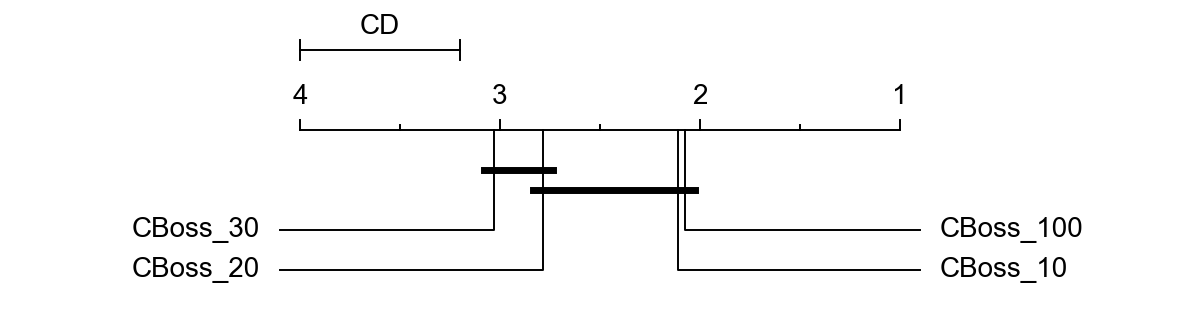
\includegraphics[width=0.49\textwidth]{cd_f_score_within_cboss.png} & & 
    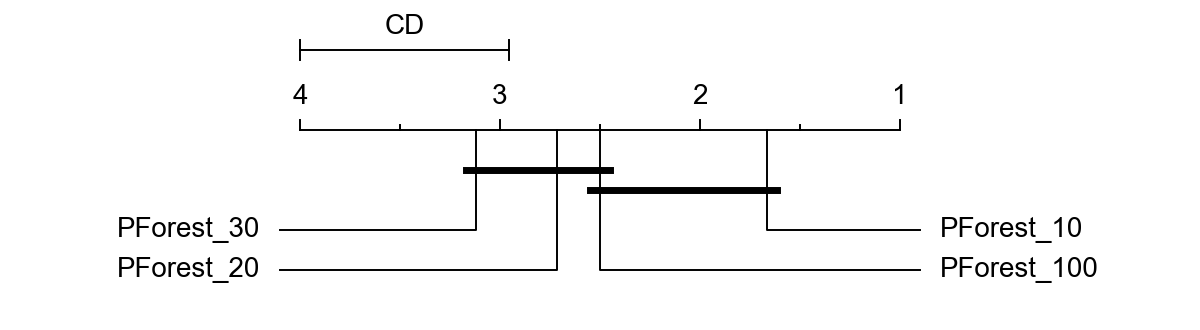
\includegraphics[width=0.49\textwidth]{cd_f_score_within_pforest.png} \\
    \textbf{(a) CBoss} & & \textbf{(b) PForest} \\[6pt]
    \end{tabular}
    \begin{tabular}{ccc}
    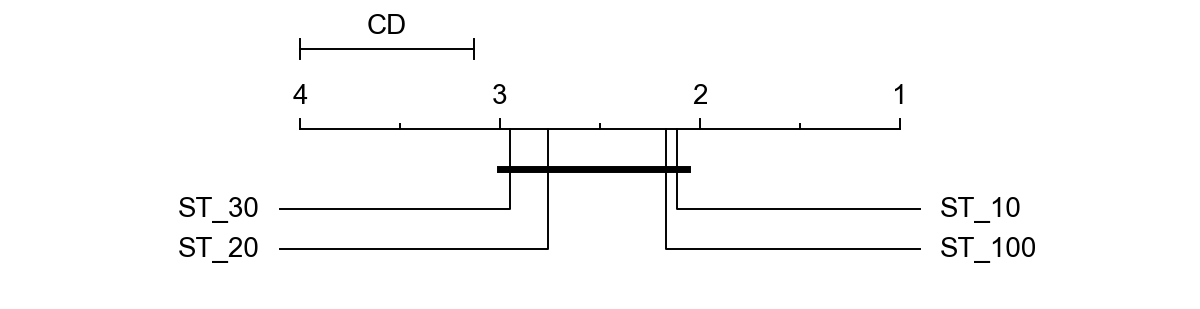
\includegraphics[width=0.49\textwidth]{cd_f_score_within_st.png} & & 
    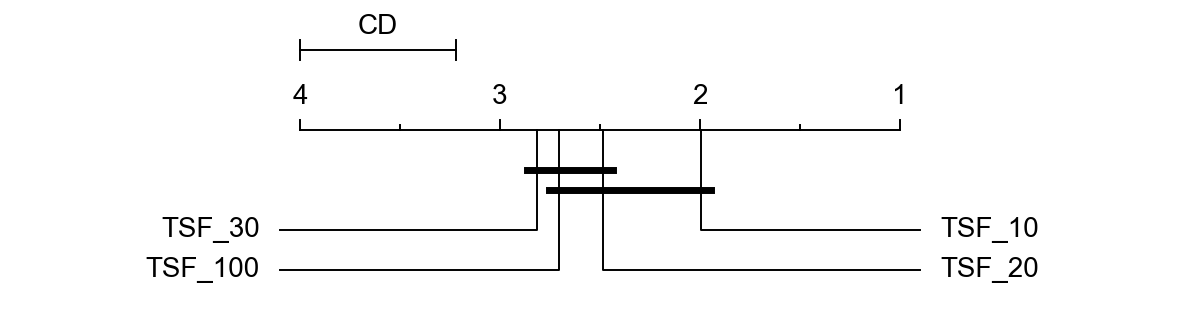
\includegraphics[width=0.49\textwidth]{cd_f_score_within_tsf.png} \\
    \textbf{(c) ST} & & \textbf{(d) TSF}  \\[6pt]
    \end{tabular}
    \begin{tabular}{ccc}
    & 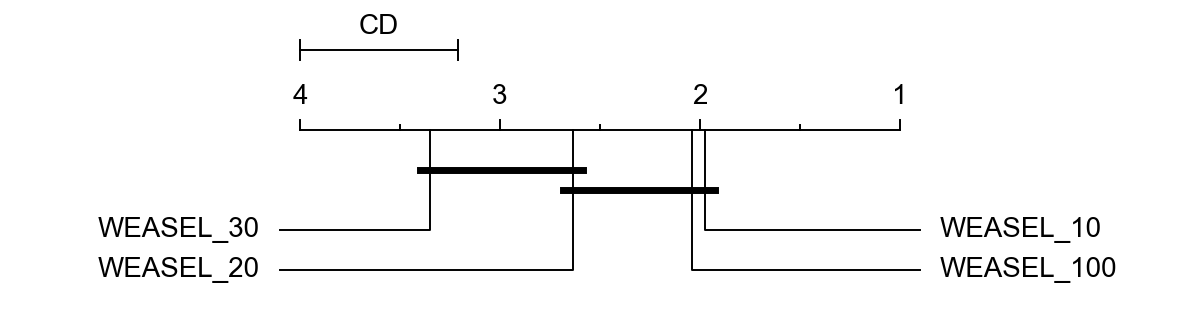
\includegraphics[width=0.49\textwidth]{cd_f_score_within_weasel.png} & \\
    & \textbf{(e) WEASEL} & \\[6pt]
    \end{tabular}
    \caption{Crtitical difference diagrams between versions of the same classifier trained on different chunks ($F_{\beta}$)}
    \label{fig:within}
\end{figure}



Figure \ref{fig:within} shows the critical difference diagram based on the $F_{\beta}$ for each classifier separately.
We compare each classifier on all the data sets that it finished across all the different chunks, regardless of the other classifiers.
The best performing algorithms lie on the right side of the diagram and the worse performing algorithms on the left side.
A bar is used to connect a clique of classifiers which are not significantly different based on their ranking. 

All classifiers show no significant difference between their 100\% classifier version and the 10\% version based on their $F_{\beta}-measure$ scores.
For CBoss, CBoss\_100 comes in the first place and CBoss\_10 comes in the second place. While for PForest, ST and WEASEL;
their respective 10\% versions; ST\_10, PForest\_10 and WEASEL\_10 rank first.
Although TSF shows no significant difference as well, but its 100\% version TSF\_100 comes in the third place.
The 20\% and 30\% versions for all the classifiers always show no difference in ranking.

If we switch to the critical difference diagrams of accuracies, we find rather different results.
Figure \ref{fig:withinacc} shows the critical difference diagrams based on the balanced accuracy for each classifier separately.

\begin{figure} [!htb]
  \centering
  \begin{tabular}{ccc}
  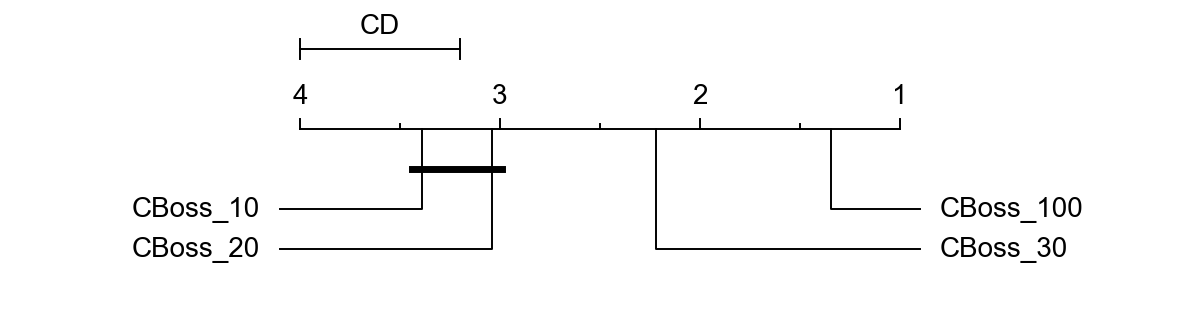
\includegraphics[width=0.49\textwidth]{cd_accuracy_within_cboss.png} & & 
  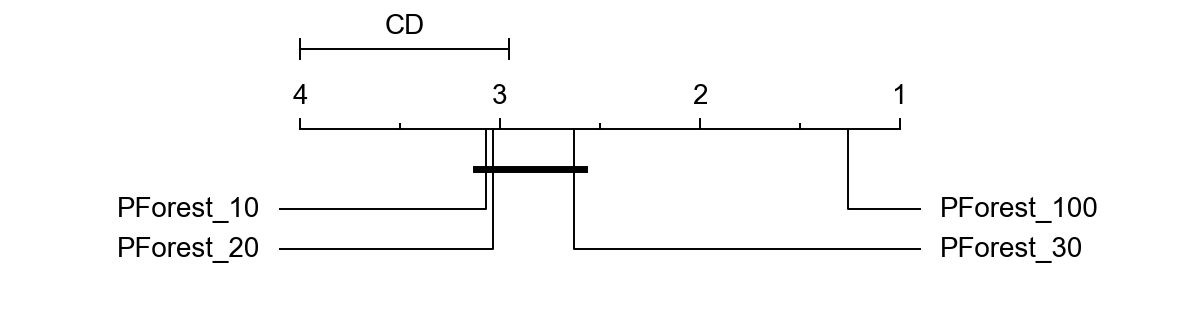
\includegraphics[width=0.49\textwidth]{cd_accuracy_within_pforest.png} \\
  \textbf{(a) CBoss} & & \textbf{(b) PForest} \\[6pt]
  \end{tabular}
  \begin{tabular}{ccc}
  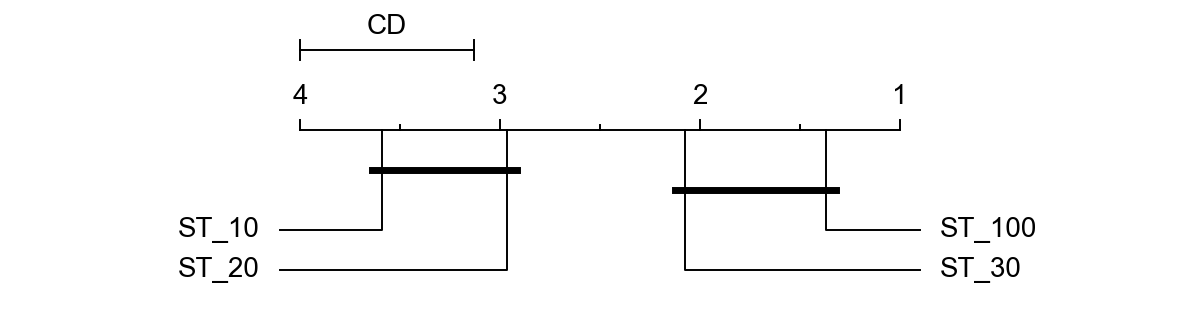
\includegraphics[width=0.49\textwidth]{cd_accuracy_within_st.png} & & 
  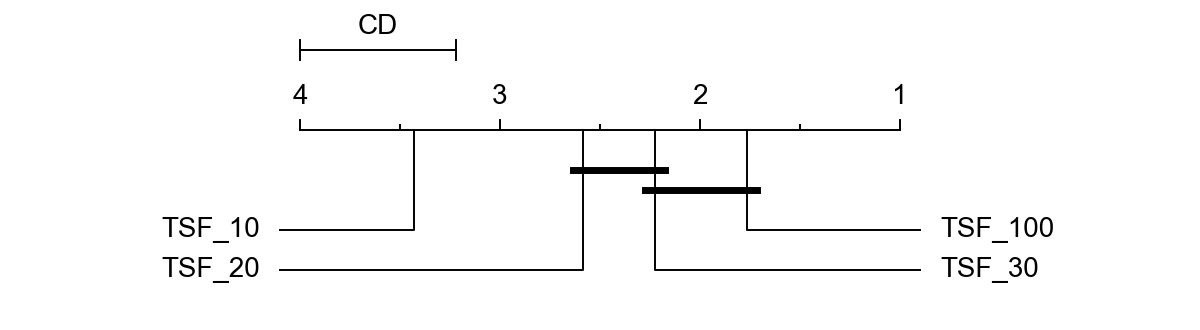
\includegraphics[width=0.49\textwidth]{cd_accuracy_within_tsf.png} \\
  \textbf{(c) ST} & & \textbf{(d) TSF}  \\[6pt]
  \end{tabular}
  \begin{tabular}{ccc}
  & 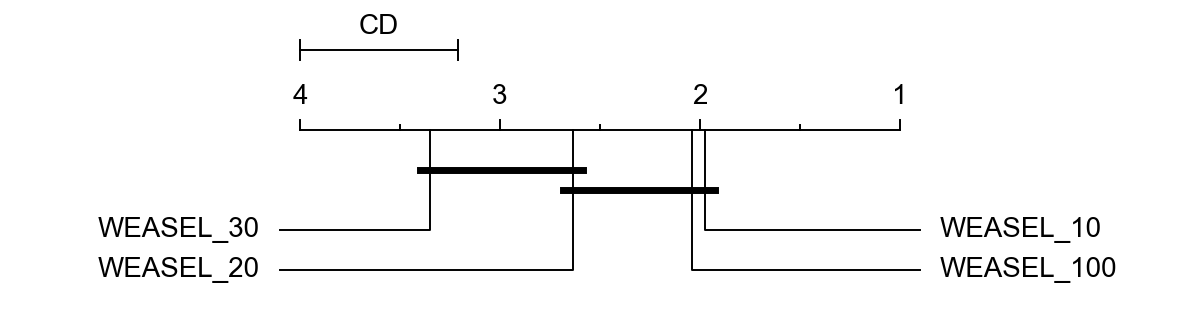
\includegraphics[width=0.49\textwidth]{cd_f_score_within_weasel.png} & \\
  & \textbf{(e) WEASEL} & \\[6pt]
  \end{tabular}
  \caption{Crtitical difference diagrams between versions of the same classifier trained on different chunks (balanced accuracy)}
  \label{fig:withinacc}
\end{figure}

For all the classifiers, the 100\% and the 10\% version are always significantly different in their ranking.
WEASEL\_100, CBoss\_100 and PForest\_100 are all significantly better than any of their other versions.
TSF\_100 and ST\_100 are ranked better than their 30\% versions TSF\_30 and ST\_30, but they are not significantly different.
This conforms with the concept of eTSC that as more data becomes available the better a classifier performs
and also demonstrates the role that earliness plays in the scores of $F_{\beta}-measure$.


\subsection{Results on Runtime Duration}
\label{SubsectionRuntime}
Another aspect we investigate for our experiments is the runtime of the classifiers.
It is not possible to carry out a comparison between the different algorithms we have used; because of the different adaptations we have applied to them.
For some classifiers, we have used an enhanced version which allows setting a contract time for feature extraction phases; like in the case of CBoss and ST.
This parameter allows us to restrict the amount of time given for the classifier.
For PForest, we have excluded two distance measures; euclidean distance because it cannot handle the early classifcation context
and TWE distance because it is the slowest elastic distance measure.
These enhancements make our results not representative for the original classifiers runtime performance.
Instead we provide information about the CPU time that was needed by each classifier to complete training on the data sets.
Figures \ref{fig:DurationCBoss}, \ref{fig:DurationPF}, \ref{fig:DurationST}, \ref{fig:DurationTSF} and \ref{fig:DurationWeasel} show the CPU time, in seconds, for the classifiers on all the used data sets.
The values represent the training time of the best model selected from the 5 cross validation folds.
If no cross validation was carried out, then the value represents the CPU time for the training process directly.

\begin{figure} [!htb]
  \centering
  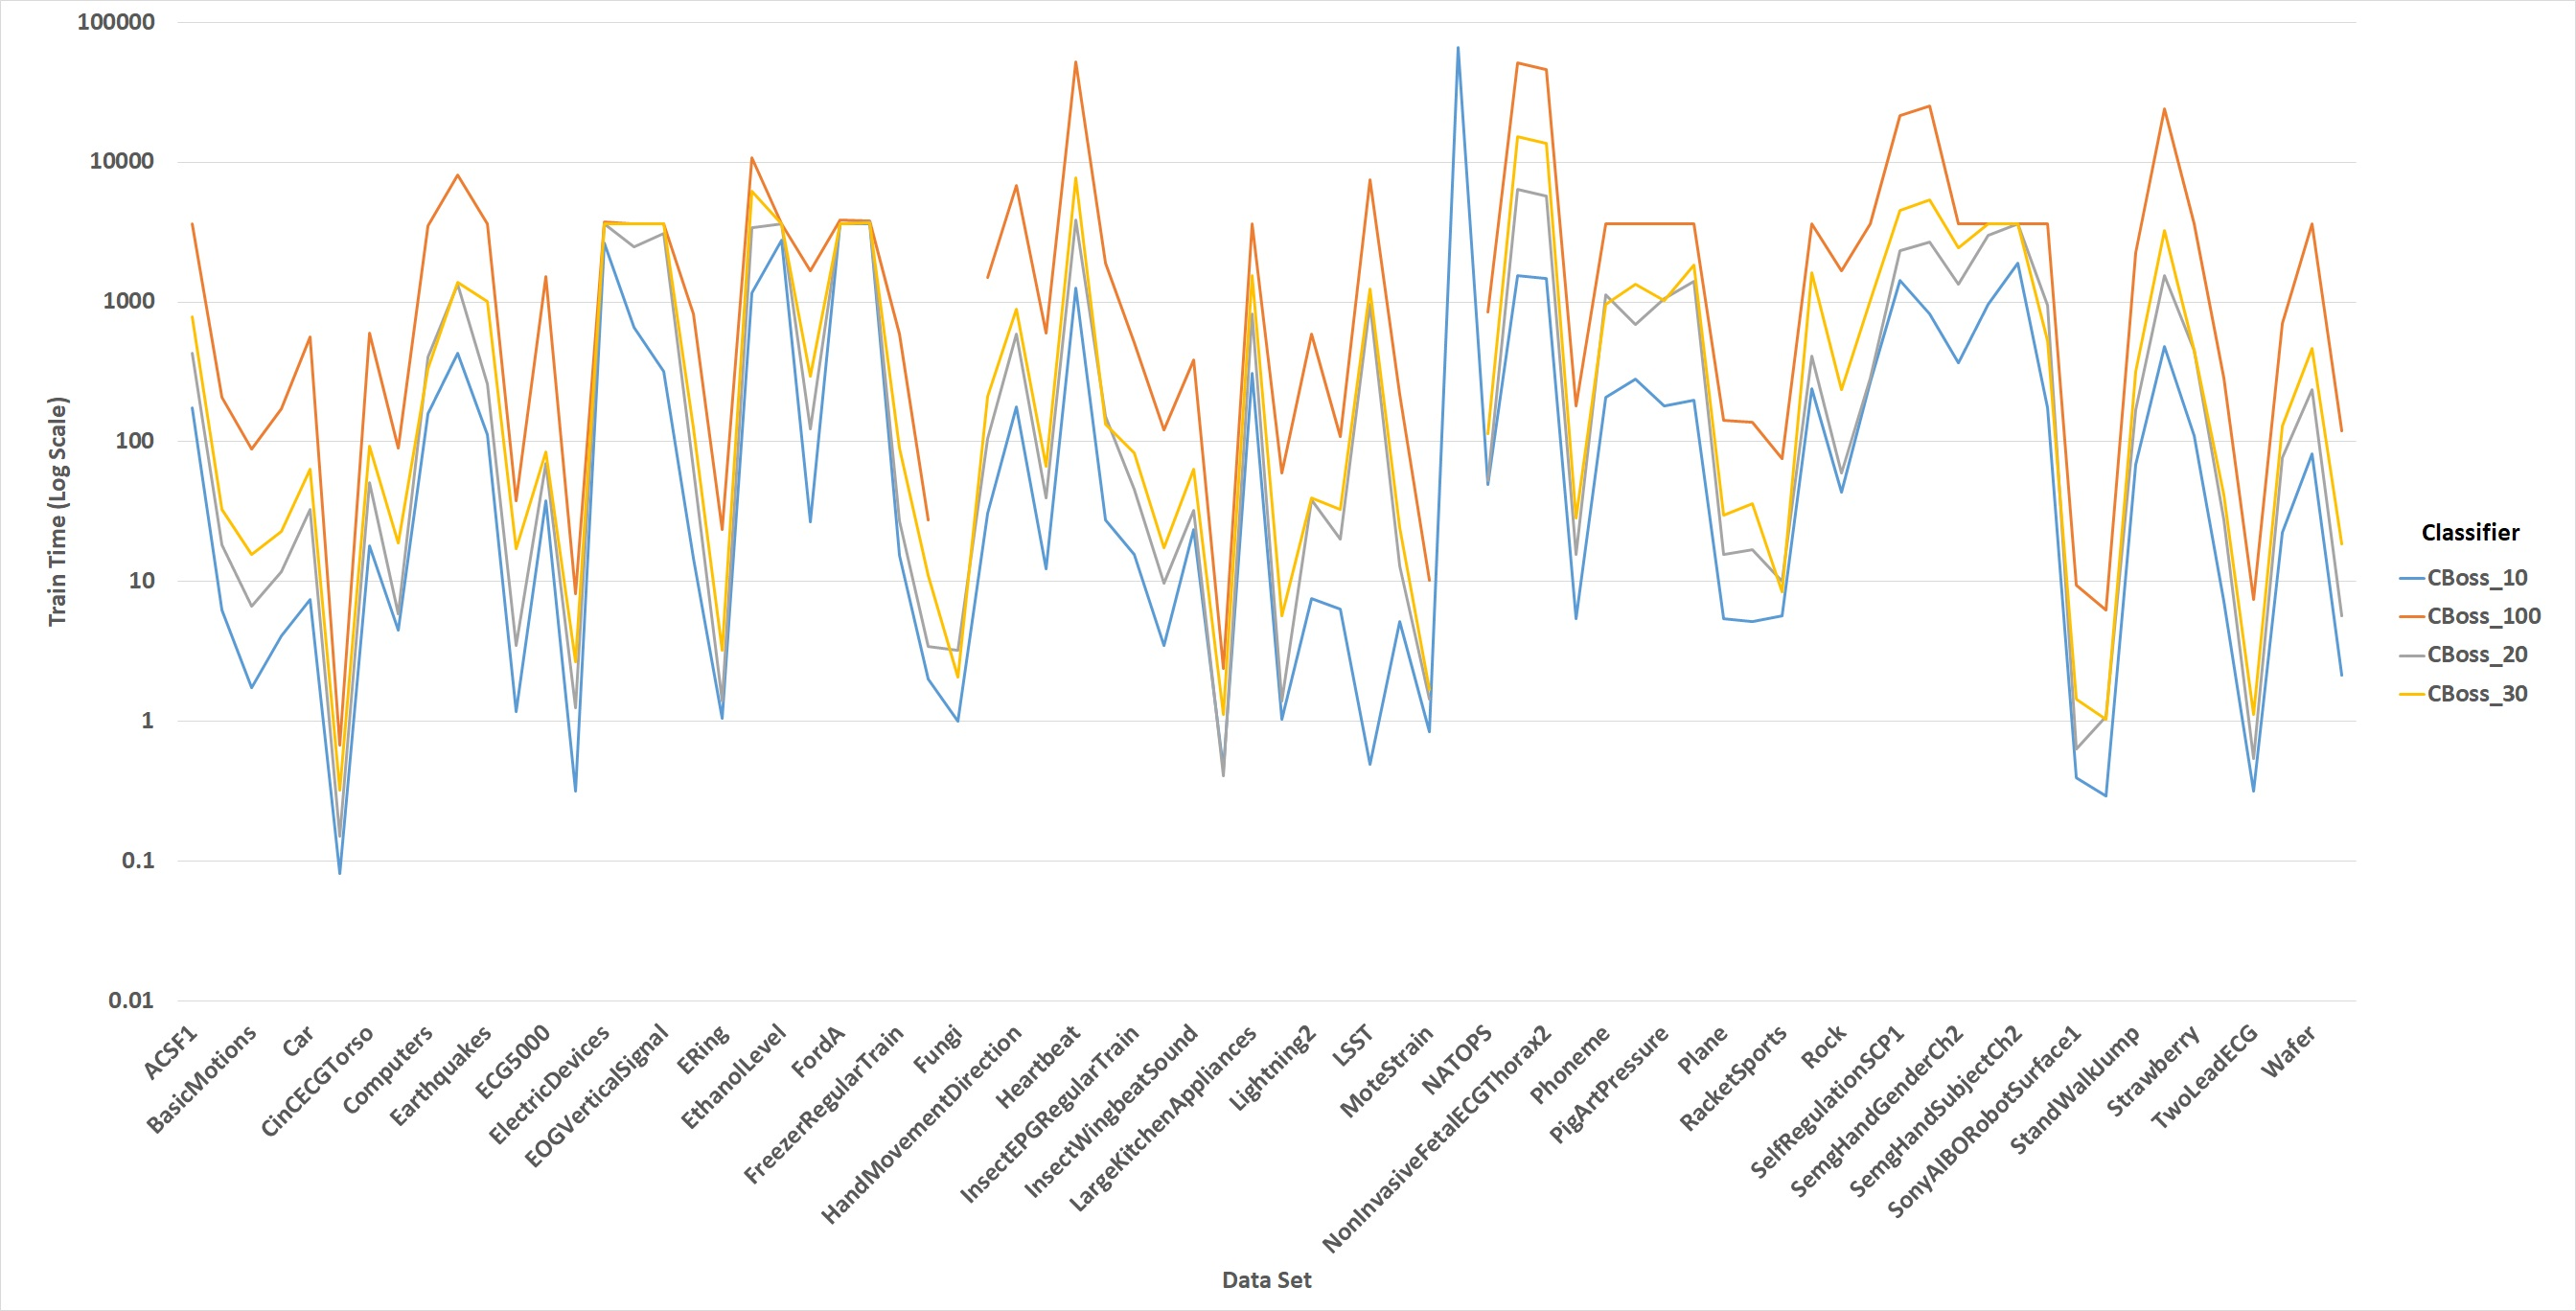
\includegraphics[width=\textwidth]{Duration_cboss.jpg}
  \caption{Train Time (CPU Time in Log Scale) for CBoss across all chunks}
  \label{fig:DurationCBoss}
\end{figure}

\begin{figure} [!htb]
  \centering
  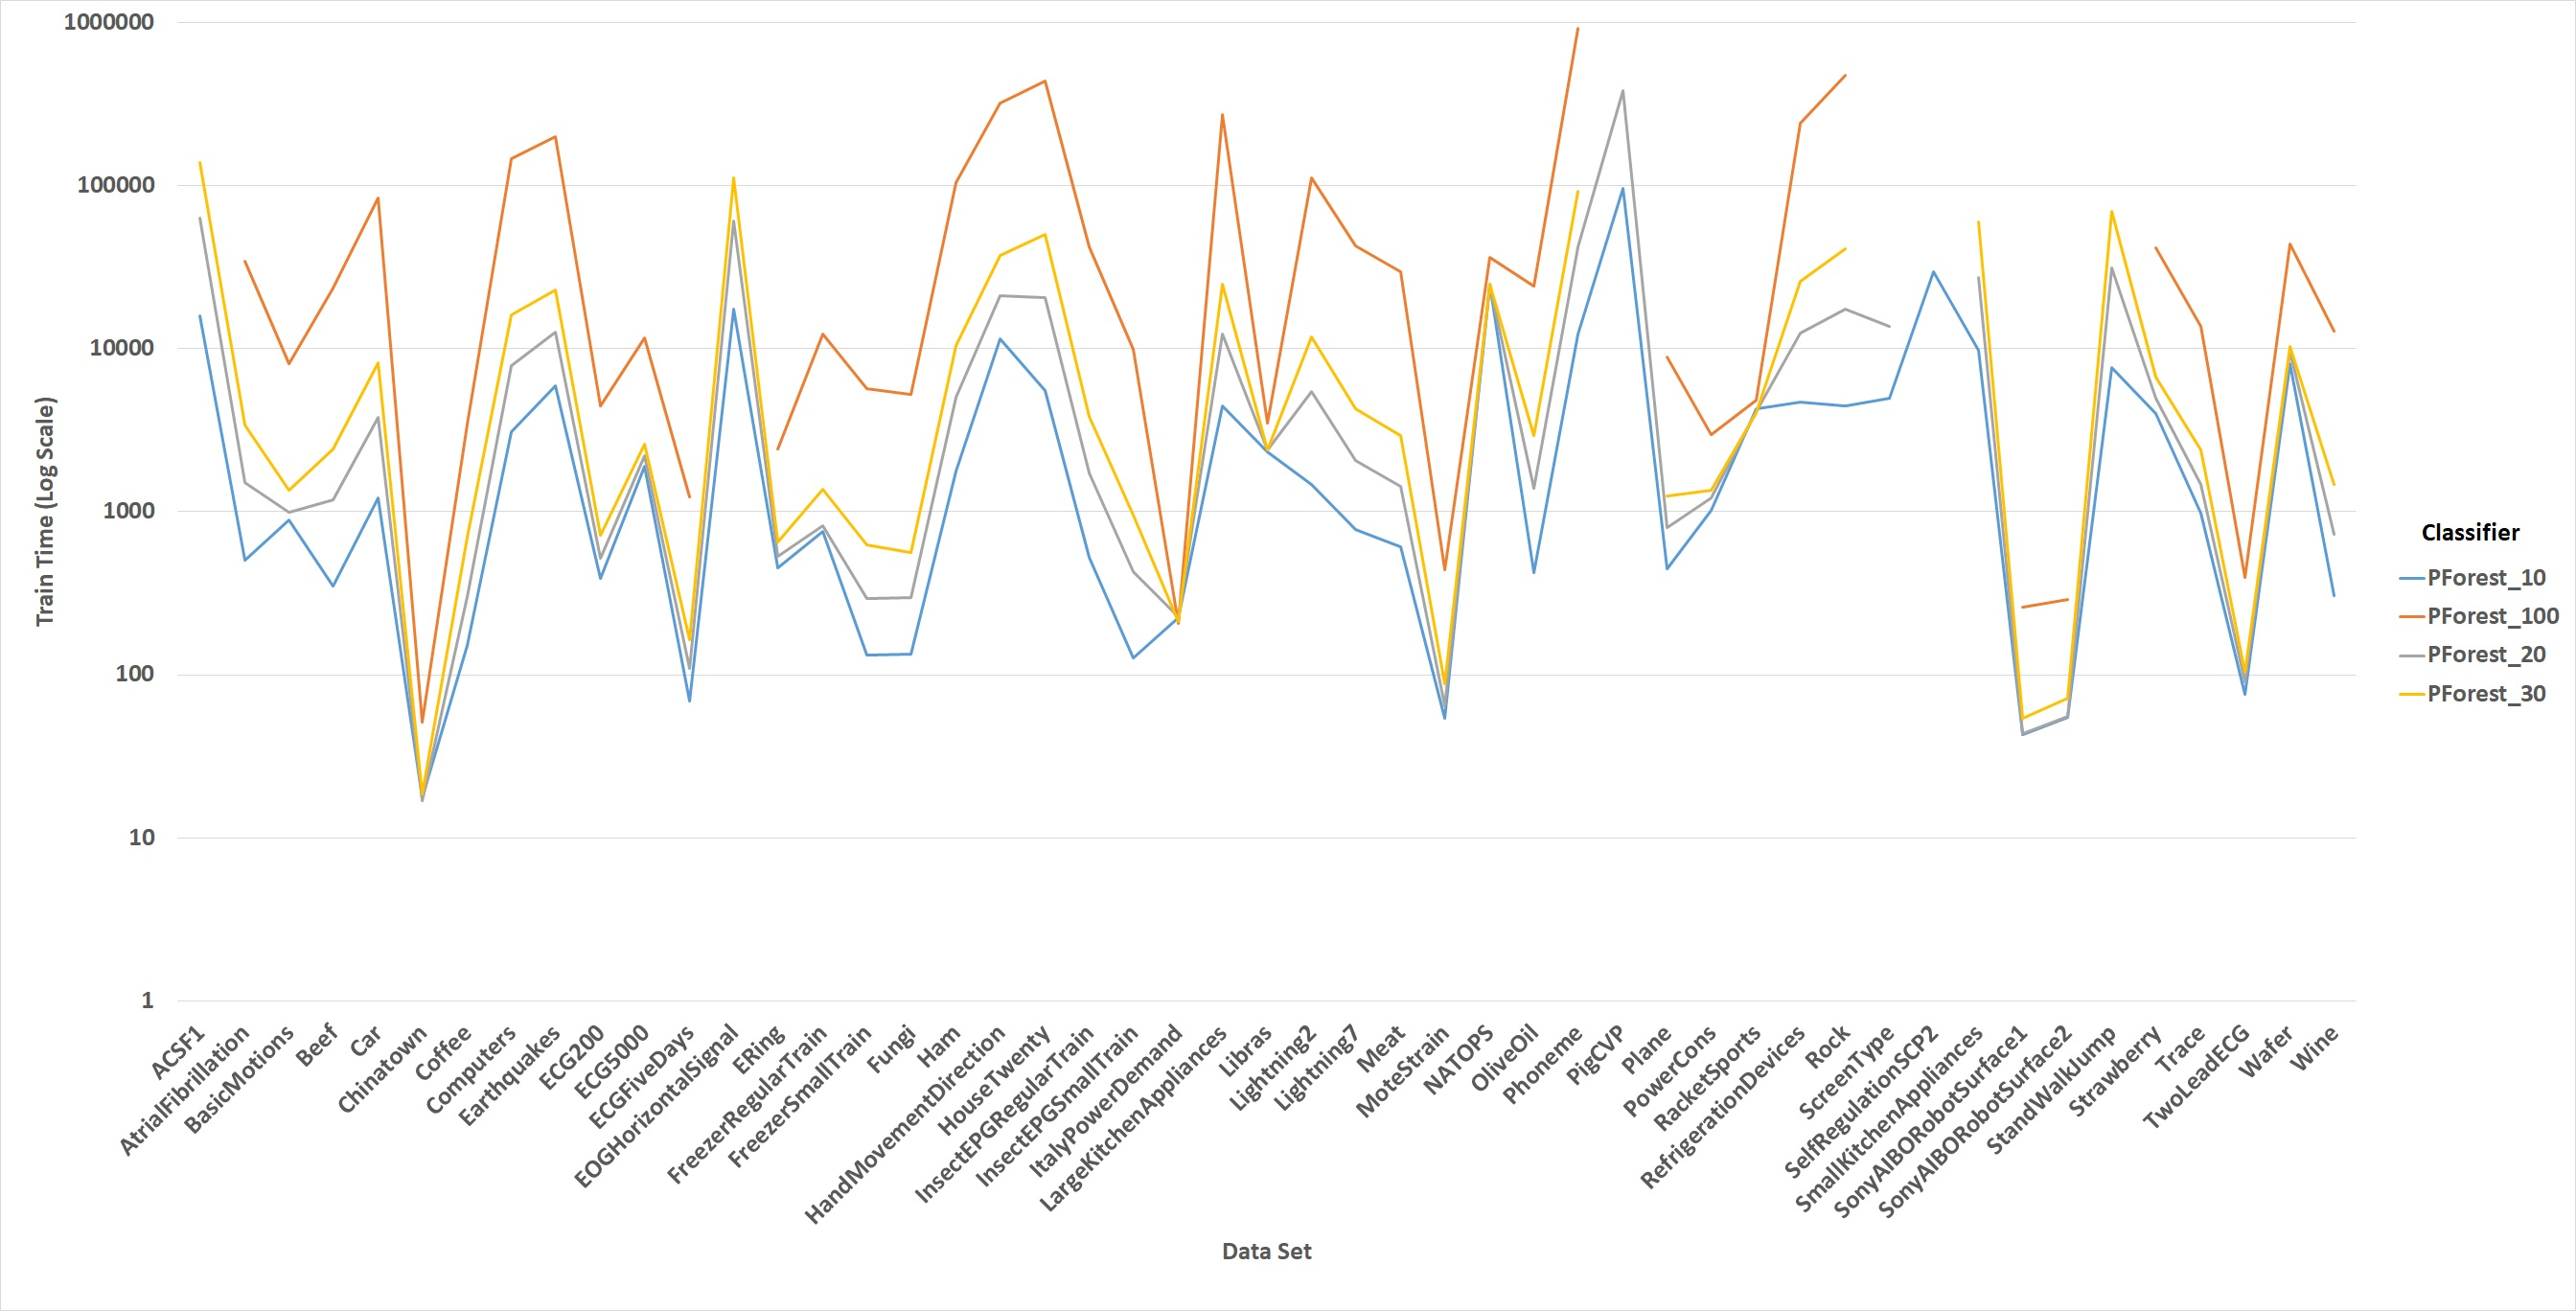
\includegraphics[width=\textwidth]{Duration_pforest.jpg}
  \caption{Train Time (CPU Time in Log Scale) for PForest across all chunks}
  \label{fig:DurationPF}
\end{figure}

\begin{figure} [!htb]
  \centering
  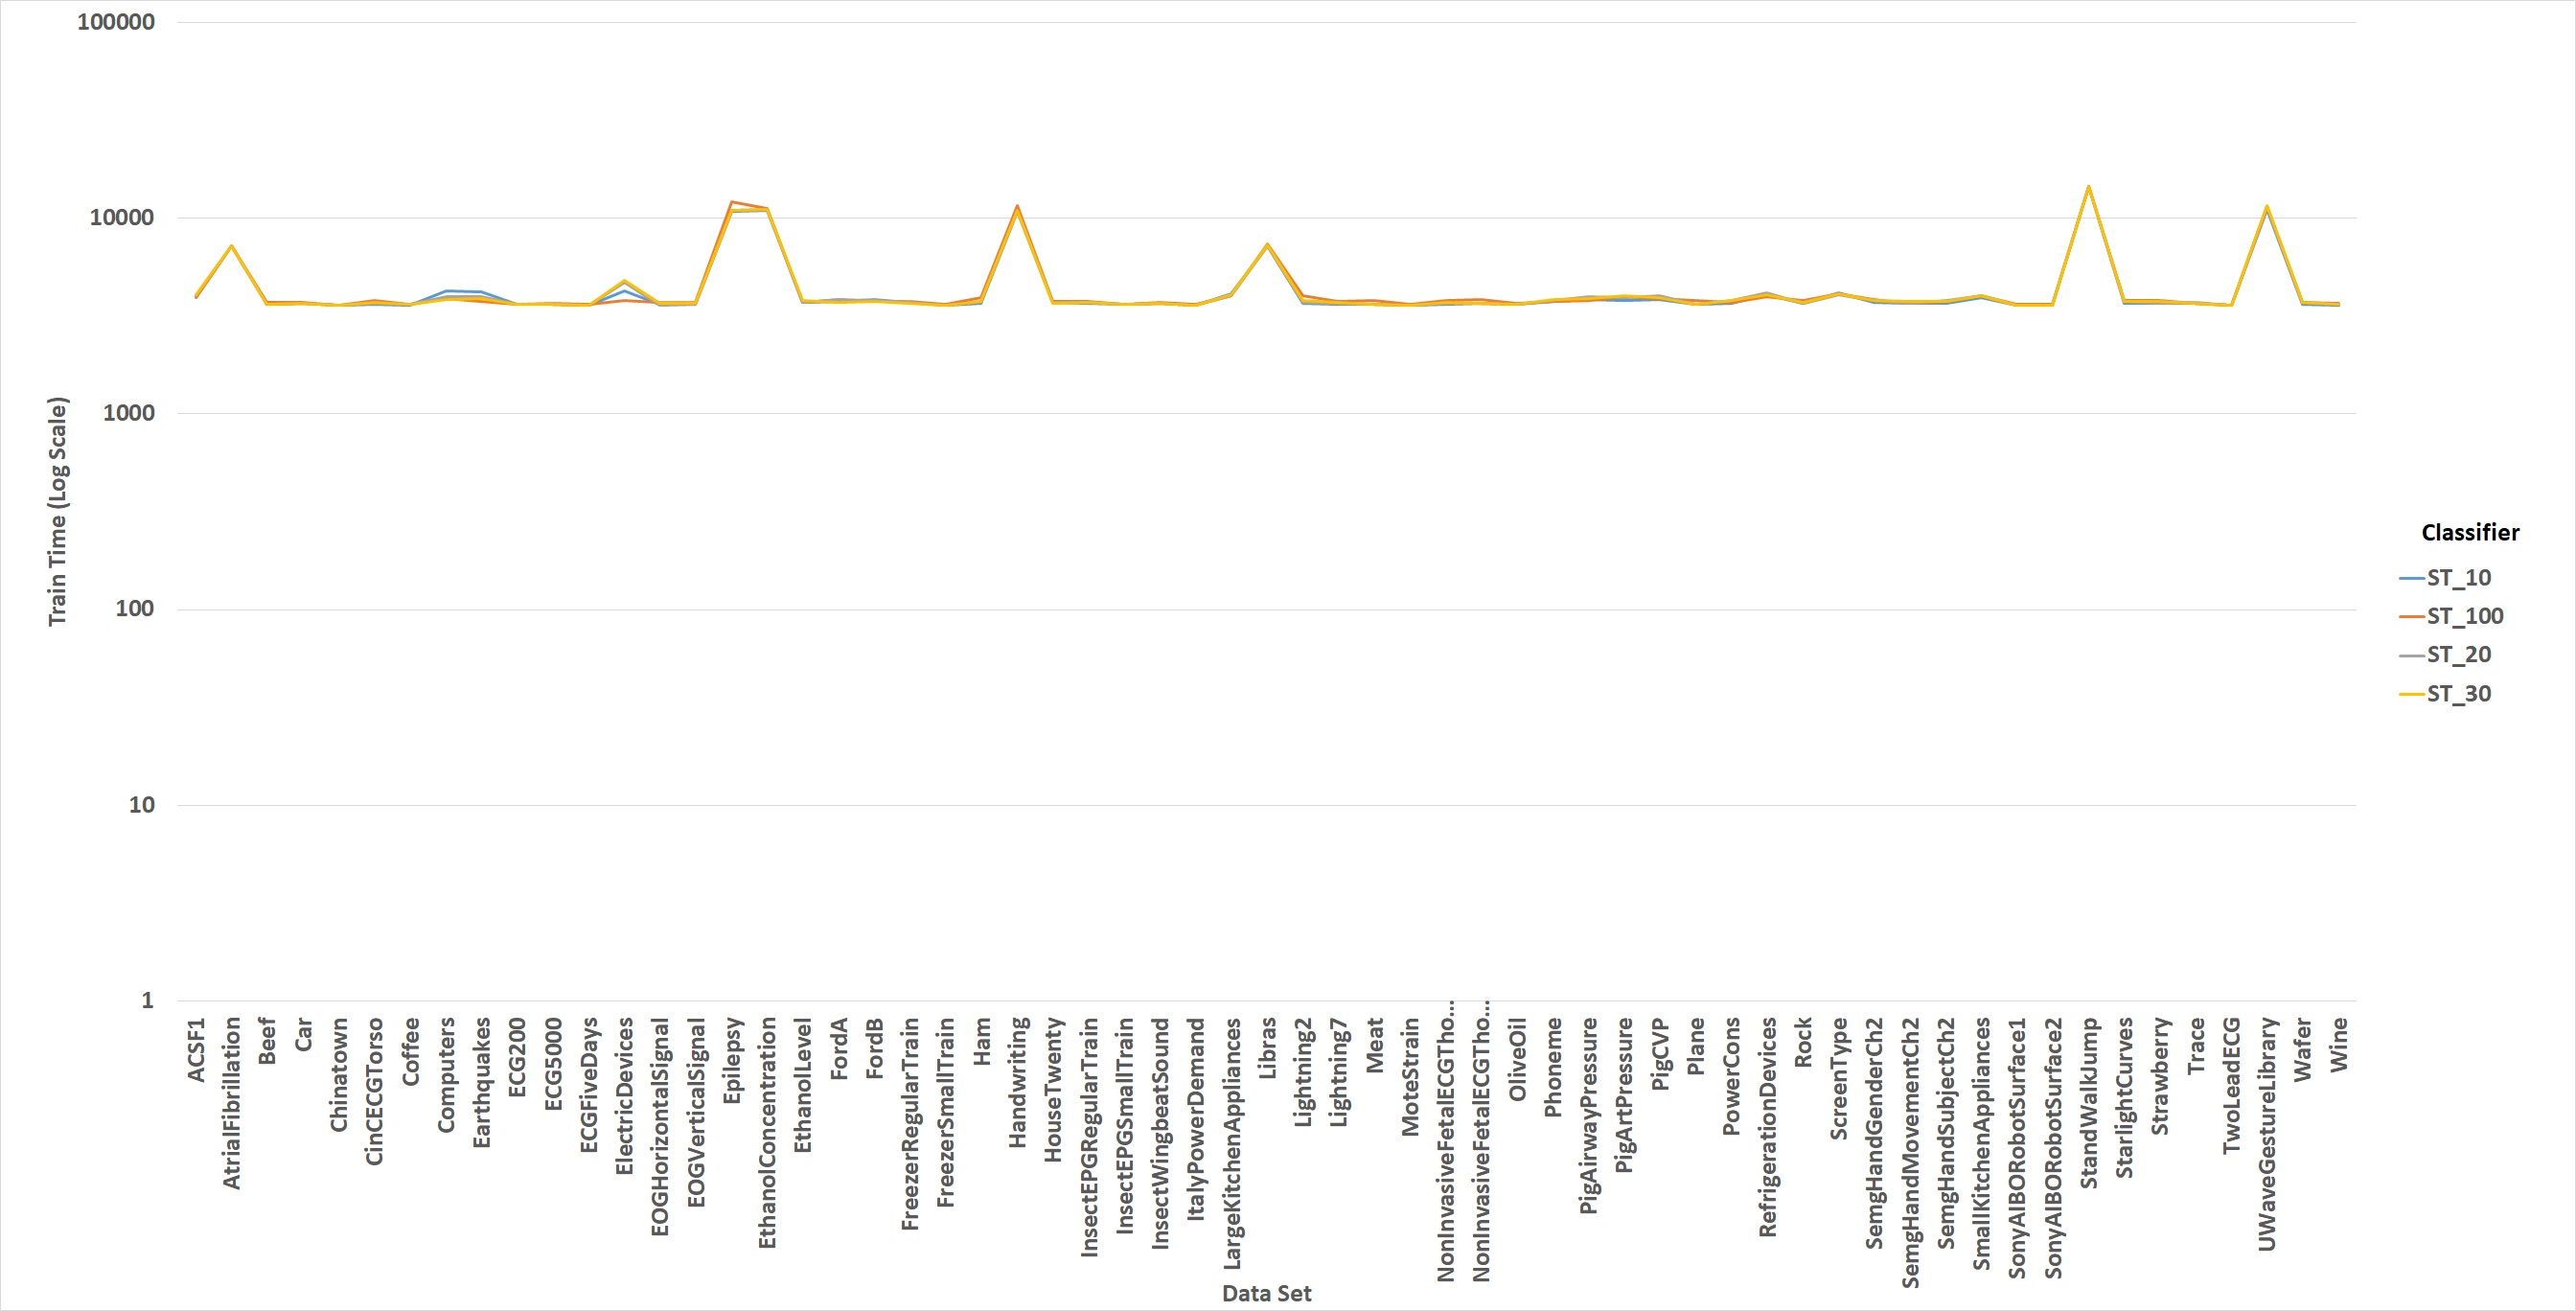
\includegraphics[width=\textwidth]{Duration_st.jpg}
  \caption{Train Time (CPU Time in Log Scale) for ST across all chunks}
  \label{fig:DurationST}
\end{figure}

\begin{figure} [!htb]
  \centering
  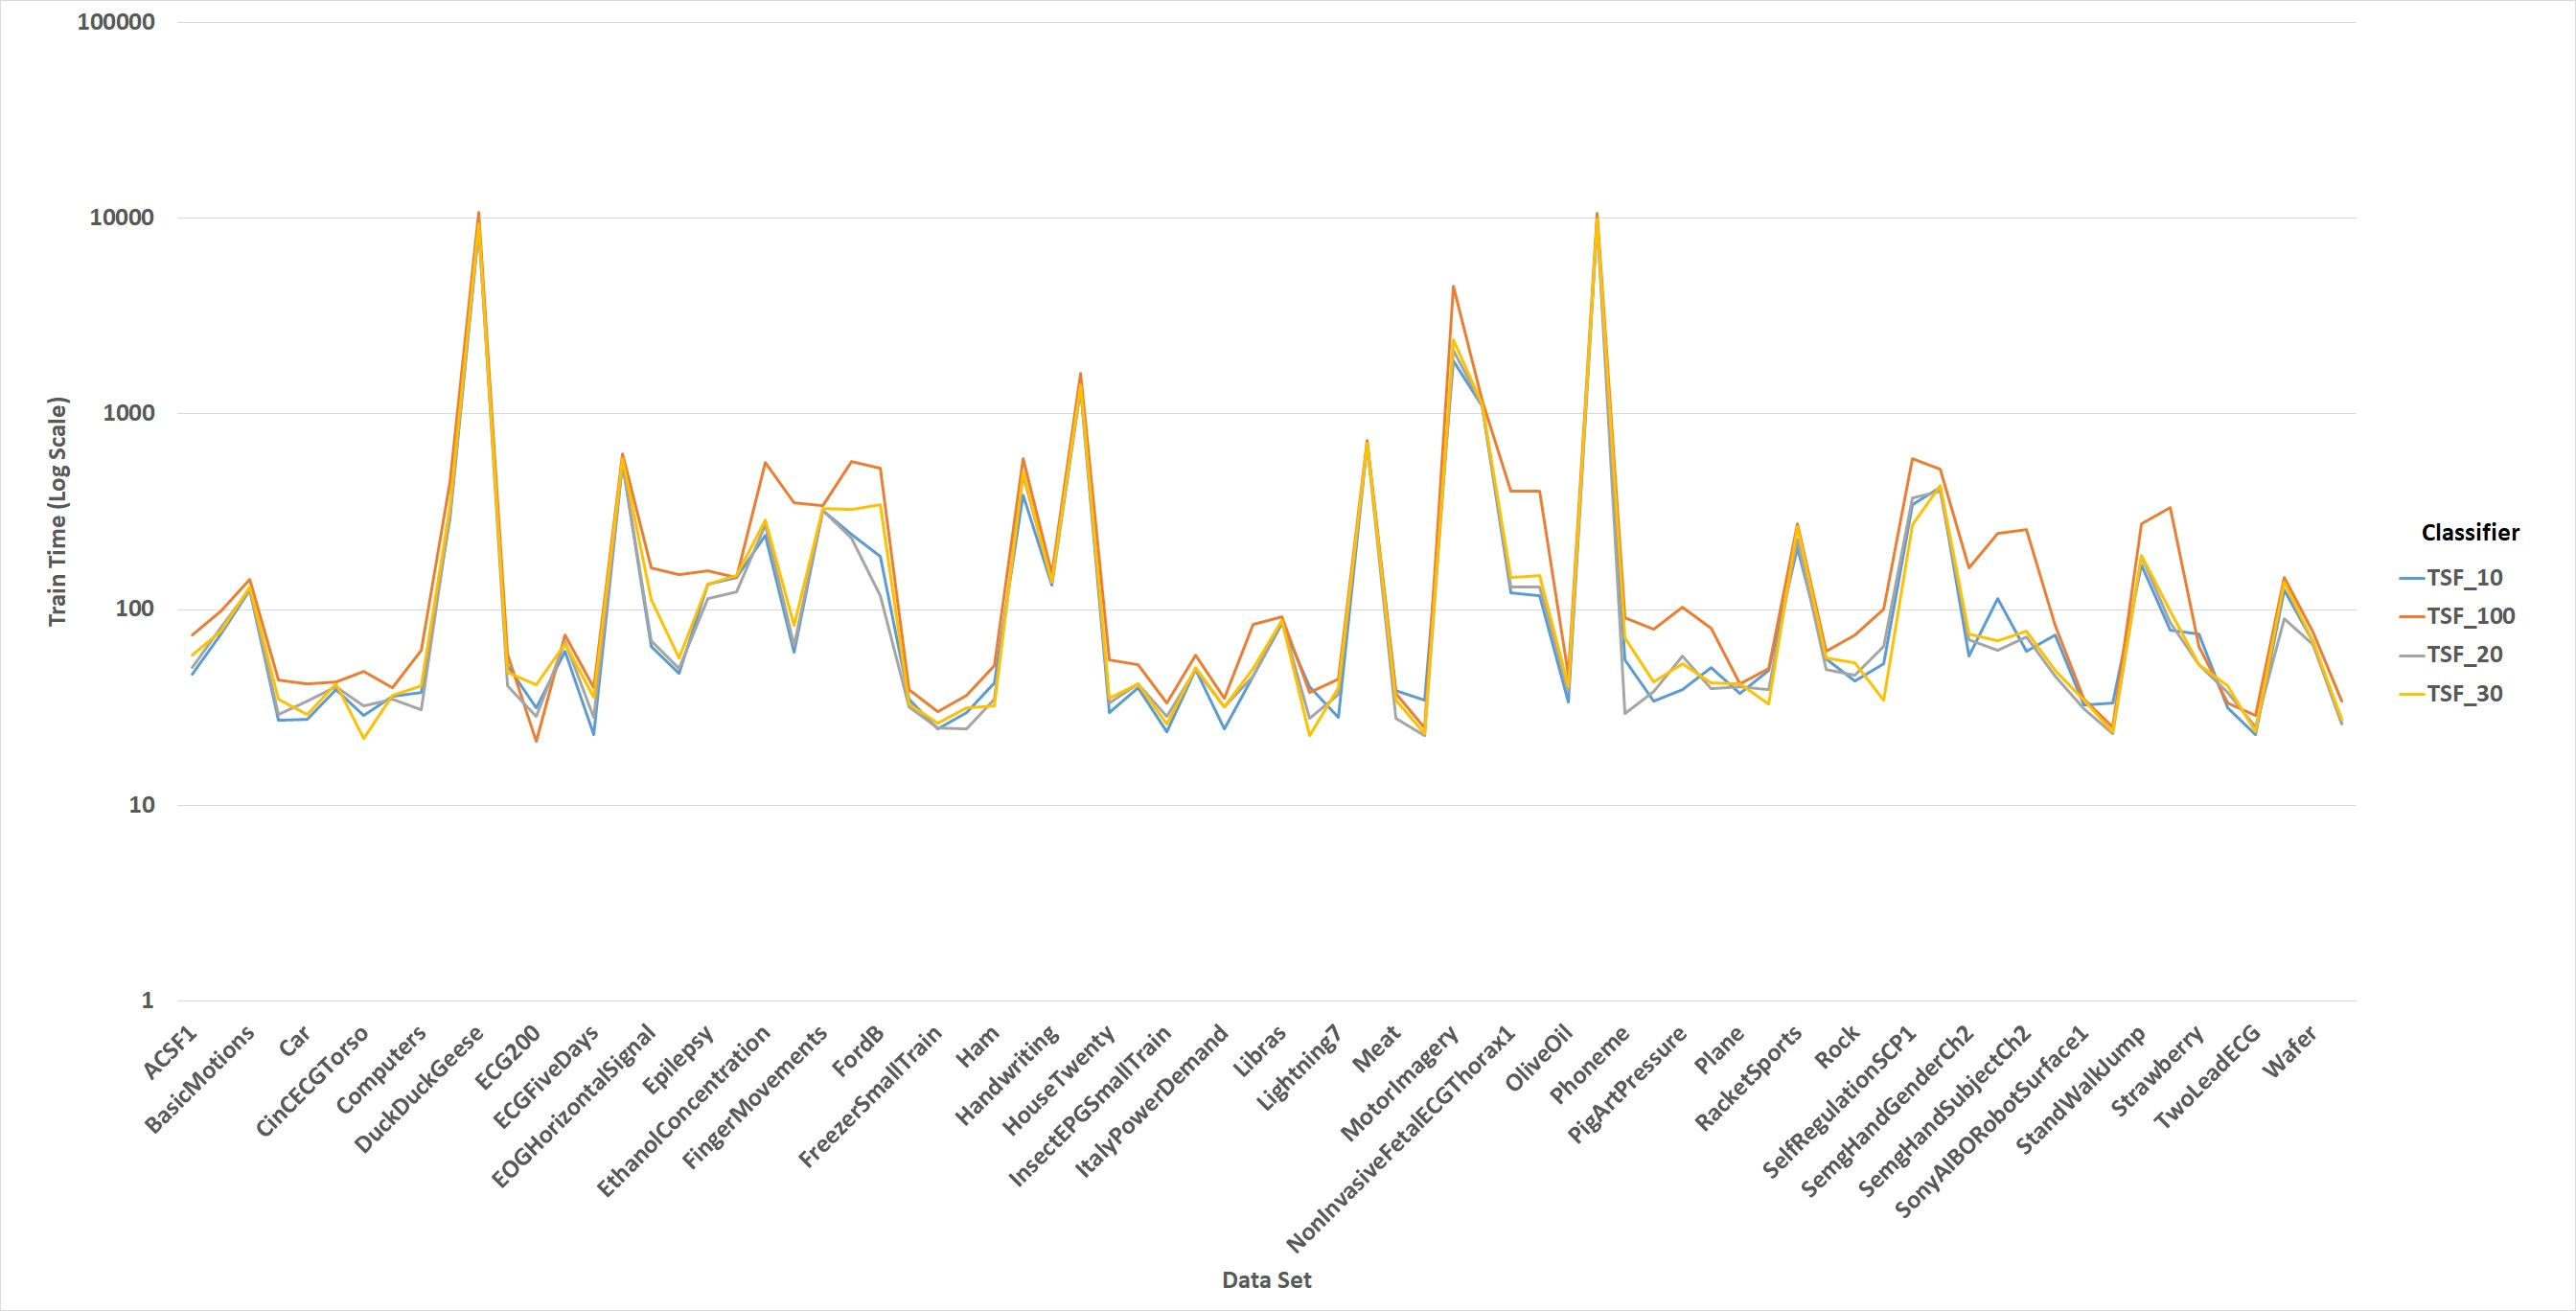
\includegraphics[width=\textwidth]{Duration_tsf.jpg}
  \caption{Train Time (CPU Time in Log Scale) for TSF across all chunks}
  \label{fig:DurationTSF}
\end{figure}

\begin{figure} [!htb]
  \centering
  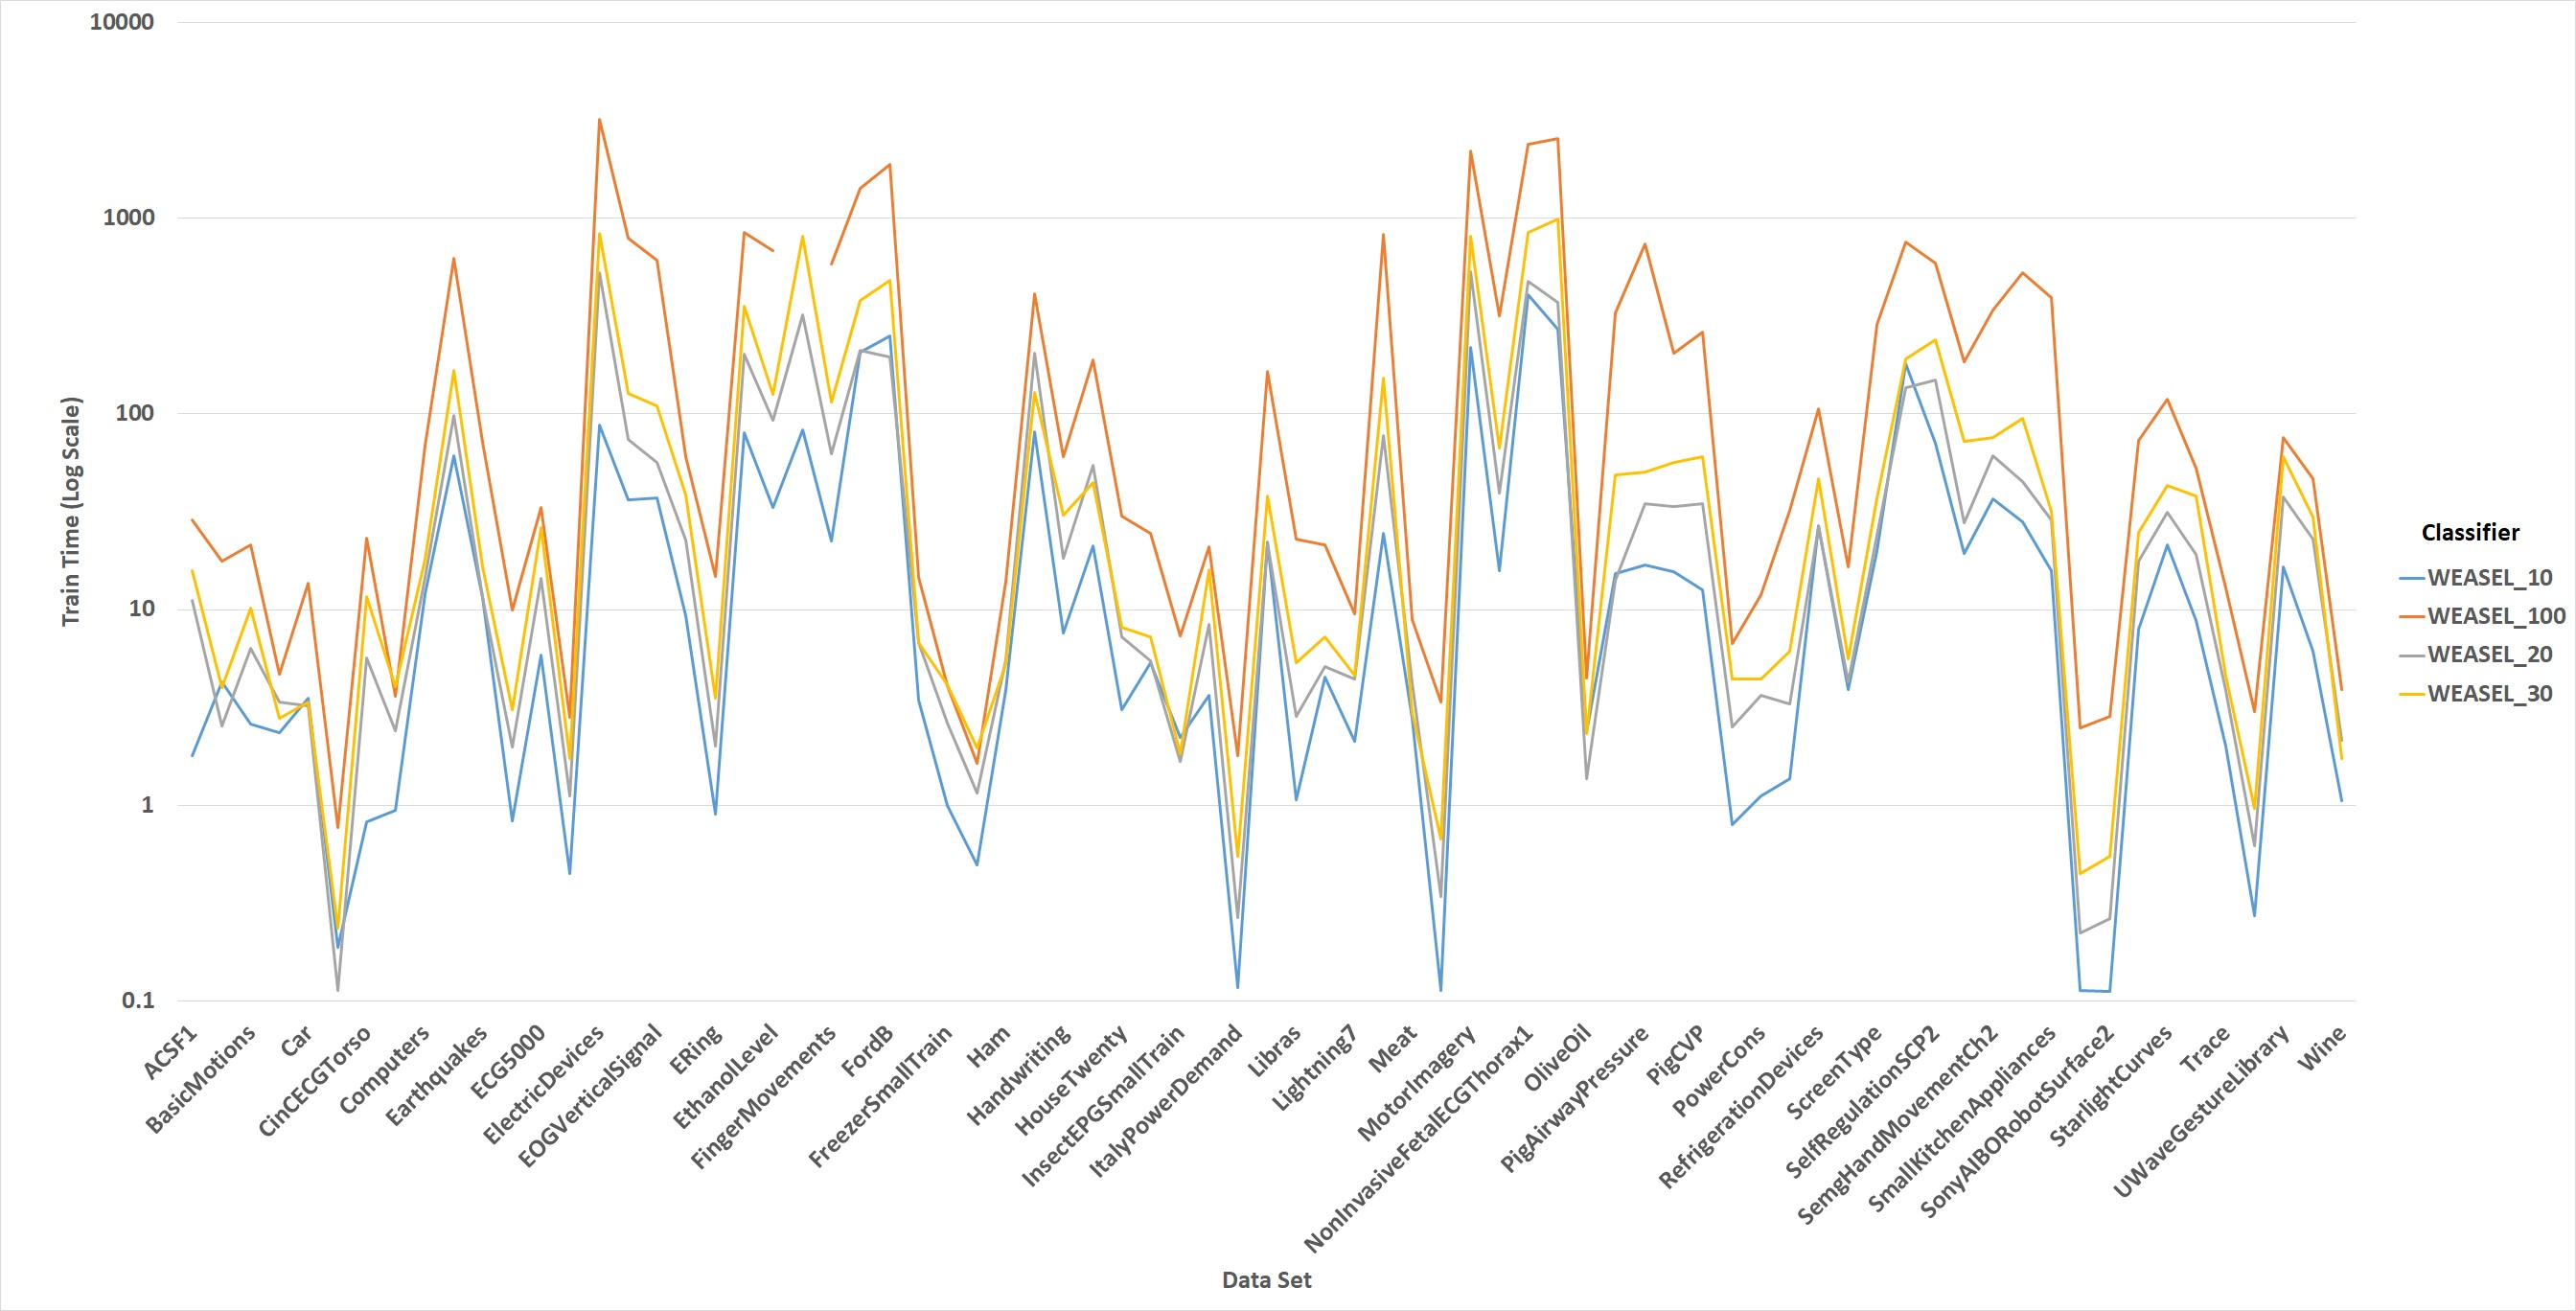
\includegraphics[width=\textwidth]{Duration_weasel.jpg}
  \caption{Train Time (CPU Time in Log Scale) for WEASEL across all chunks}
  \label{fig:DurationWeasel}
\end{figure}

TSF and WEASEL have short training durations. TSF doesn't use any complex features and instead depends on simple summary statistics on intervals.
The stochastic selection of intervals speeds its learning process even faster.
WEASEL on the other hand is designed for speed and quality, but this comes on the expense of memory.
Although WEASEL takes short training times, it has failed to complete on some data sets due to its large memory print.
ST is known to be a strong but rather a significantly slow classifier.
The use of the contractable version of ST clearly pays off, it stabilizes the training time across the different chunks by limiting the time during which ST looks for shapelets.
The slowest classifier among all experiments was PForest. We provide train time results and breakdown by data characteristics in appendix \ref{AppendixDuration}

\section{Recommender Results}
\label{SectionRecommenderResults}
We divide our results for the recommender into two main parts. The first part presents the results for the chunk learners, while the second part presents the results for the final recommendation of the whole recommender.
In the chunks learners results part, we discuss the performance of each chunk learner and the important features for building the random forests.
In the final recommendation part, we discuss the overall performance of the recommender based on its ability to correctly suggest good performing classifiers.

\subsection{Are the chunk learners able to learn F-scores for the classifiers ?}
\label{SubsectionFScoreResults}
% results for f-score
Table \ref{TableOverallErrors} shows the overall performance of the chunk learners across all 50 runs.
In general, the chunk learners are able to learn about the performance of classifiers on the different chunks, but their mean errors are relatively high.
As evident from the results, there is an inverse relation between the performance of the chunk learners and the revealed\%.
The chunk learner that trains on the 10\% data is able to score the best scores across all the chunk learners.
The more revealed data, the harder it becomes for the chunk learners to accurately predict performance of classifiers.

\begin{table}[hp!]
    \setlength\extrarowheight{2pt} % for a bit of visual "breathing space"
    \begin{tabularx}{\textwidth}{|X|X|X|}
    \hline
    \textbf{Revealed\%} & \textbf{Avg MAE} & \textbf{Avg RMSE} \\ \hline
        10 & 4.82 & 6.71 \\ \hline
        20 & 9.57 & 12.42 \\ \hline
        30 & 12.03 & 15.46 \\ \hline
        100 & 15.58 & 19.52 \\ \hline
      \caption{Overall performance of chunk learners in predicting actual $F_{\beta}$ scores over 50 runs}
      \label{TableOverallErrors}
      \end{tabularx}
  \end{table}

Figure \ref{Img:HistogramRMSE} gives a more detailed view of the distribution of RMSE for the chunk learners.
It is clear that not only the curves of the higher chunk learner shift towards higher error values, but also the spread of the values is wider.
This indicates that few of the predictions made by the lower chunk learner are significantly worse than their actual values.
While the higher chunk learner is generally worse and makes larger mistakes by predicting values that are clearly worse than the actual performance of the classifiers.

  \begin{figure}[hp!]
    \captionsetup{justification=raggedright}
    \centering
    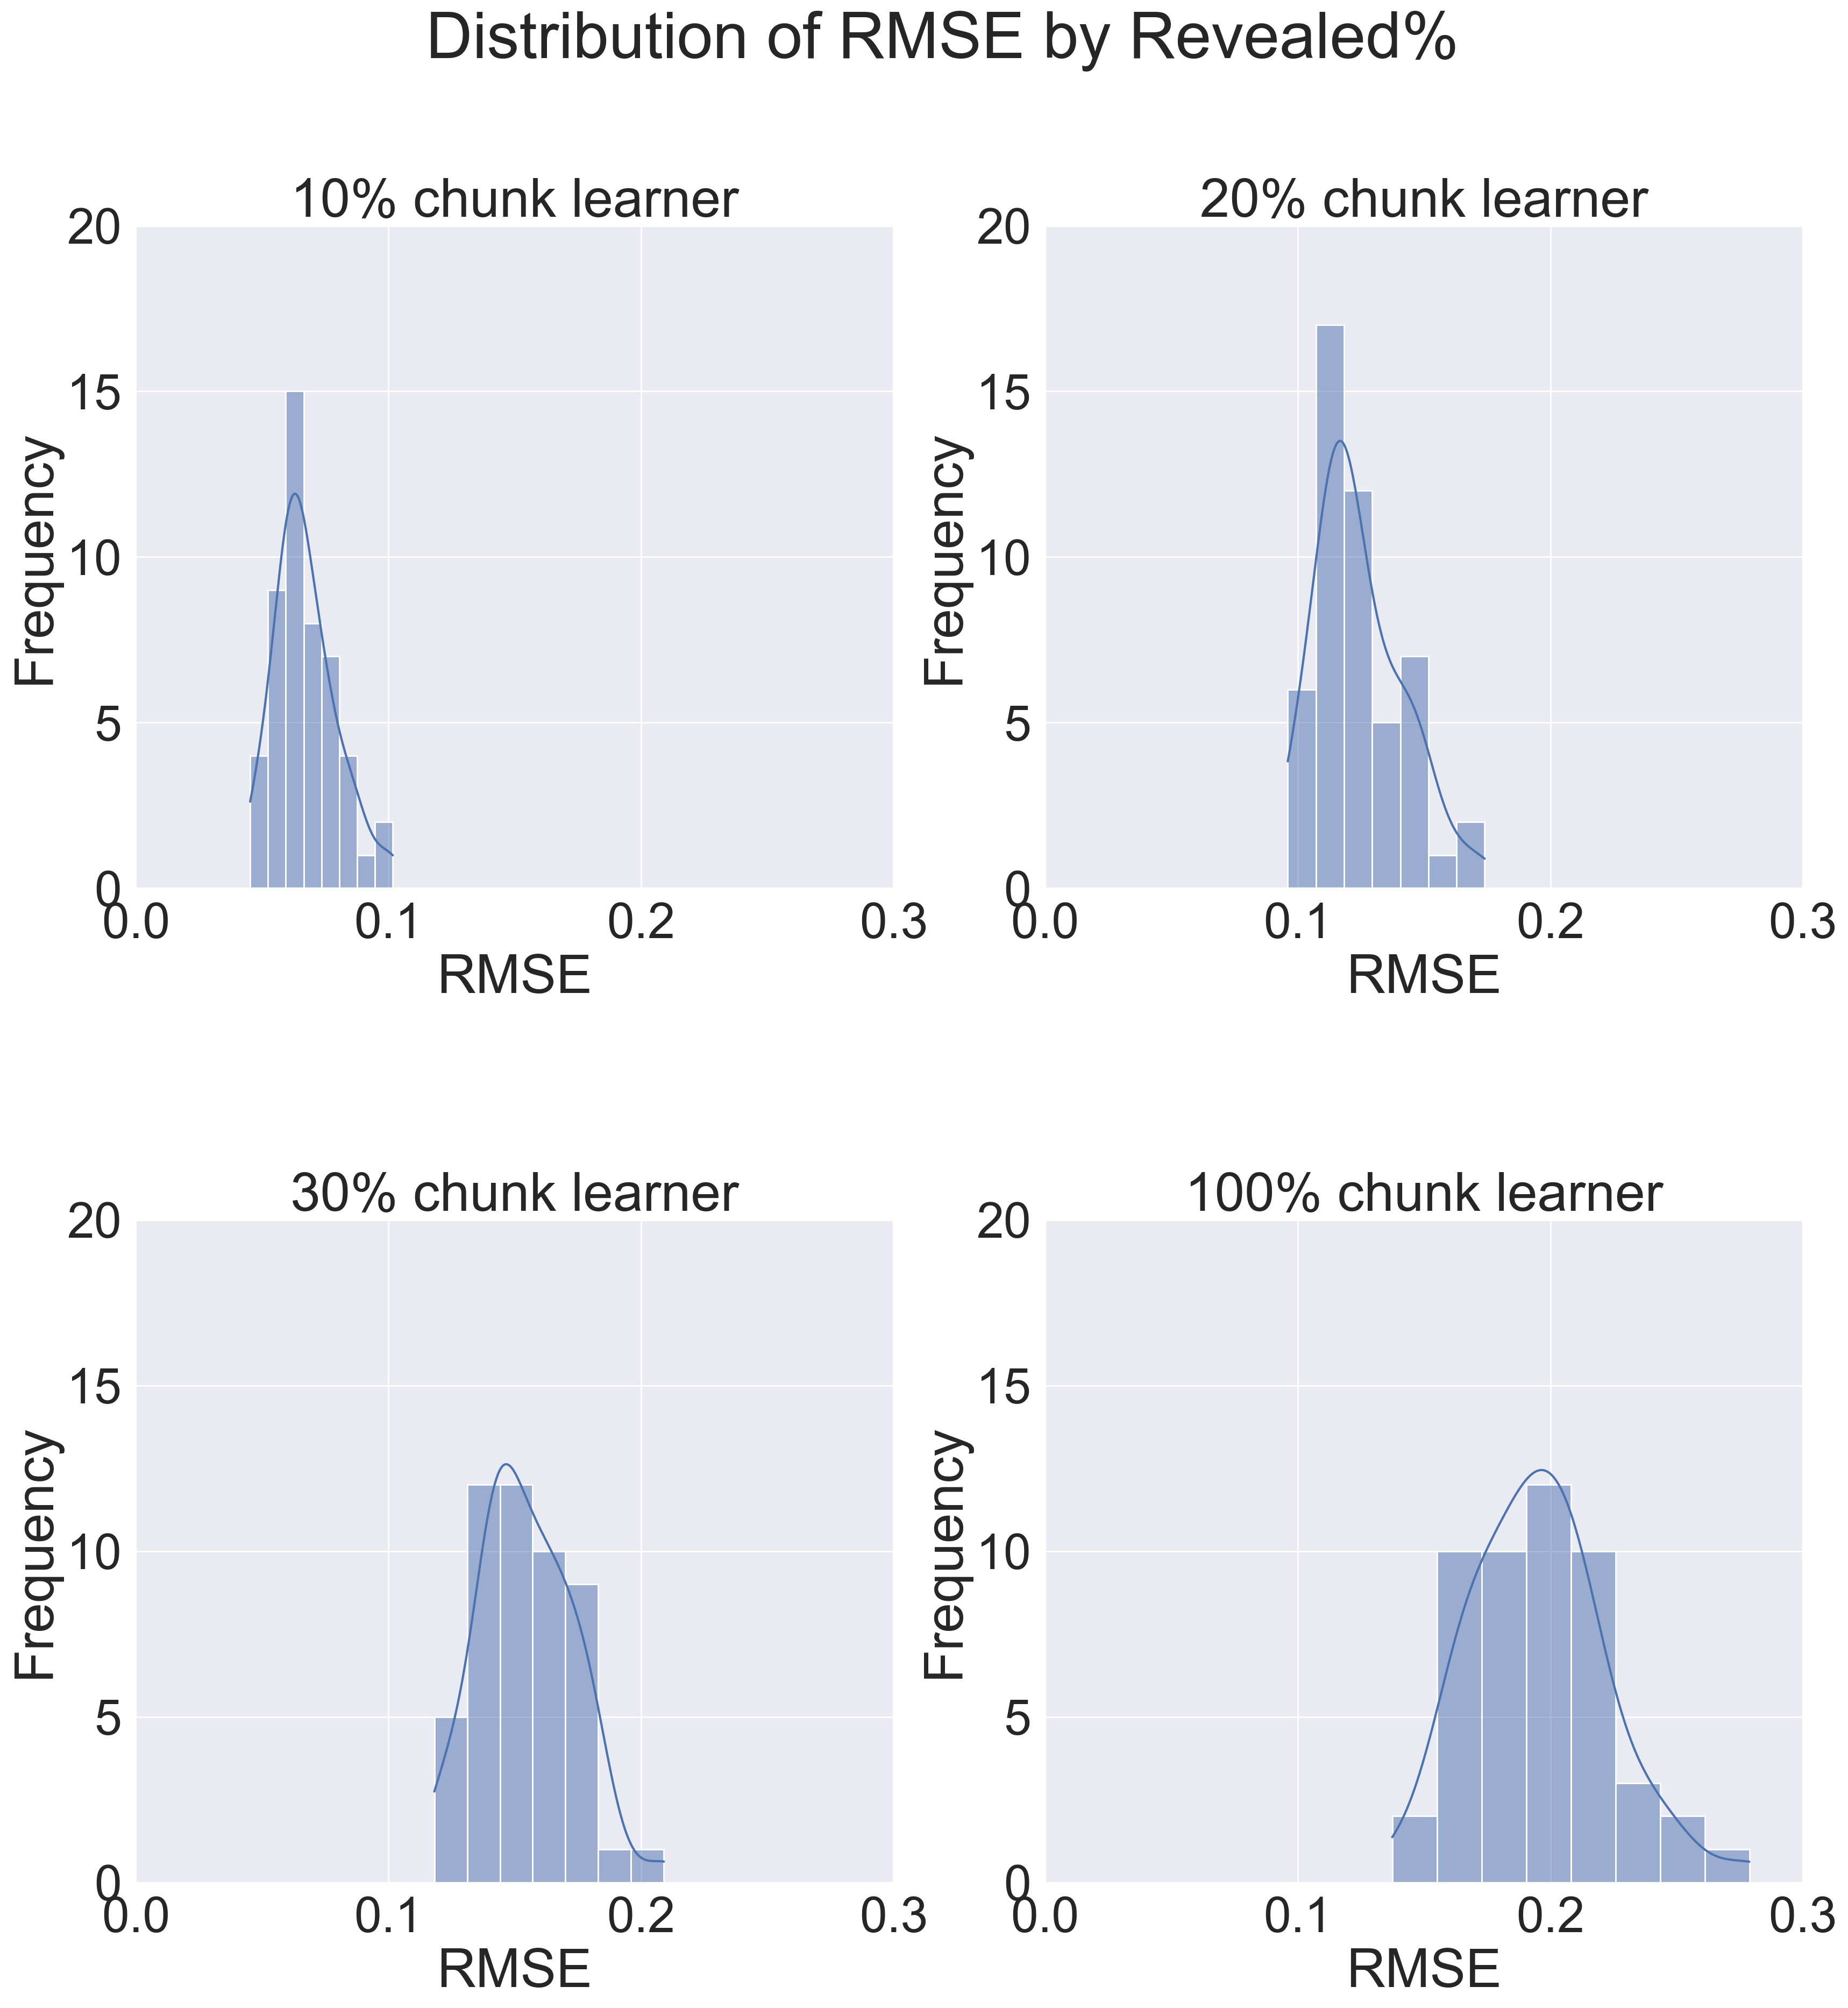
\includegraphics[width=\textwidth]{hist_rmse.jpg}
    \centering
    \caption{Histograms for distribution of RMSE per chunk over 50 runs}
    \label{Img:HistogramRMSE}
  \end{figure}

Figures \ref{Img:MAEClassifier} and \ref{Img:RMSEClassifier} visualize the MEA and RMSE of each chunk learner per classifier.
It is evident from the results that for CBoss, ST and WEASEL; the chunk learners are able to score better results as more data is revealed.
It is the opposite scenario for PForest. The first 3 chunk learners score the least errors for PForest, but on the 100\% dara the errors significantly increase to be the worst among all.
This explains the the long tail that appears in the 100\% chunk learner RMSE histogram due to the large differences between the actual and predicted F-scores for PForest on the 100\% data.

  \begin{figure}[hp!]
    \captionsetup{justification=raggedright}
    \centering
    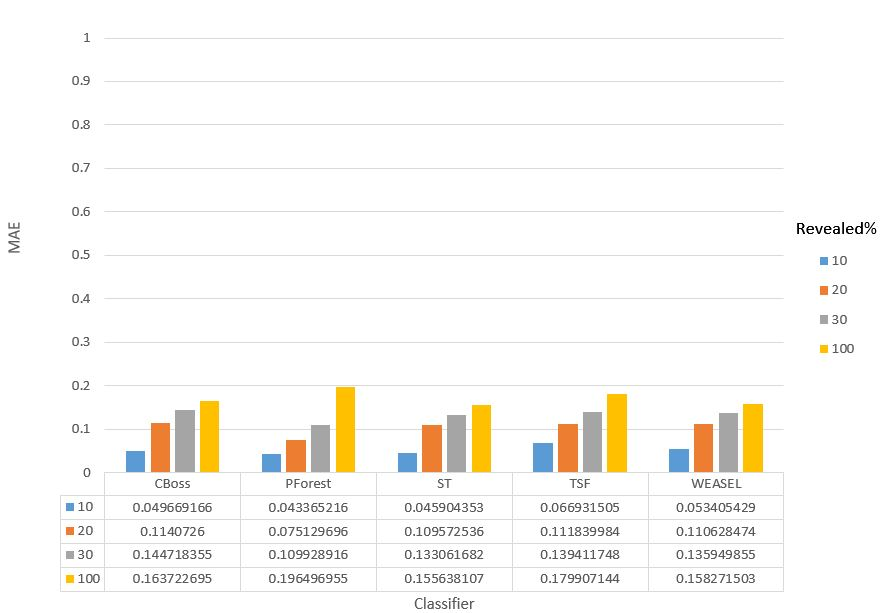
\includegraphics[width=\textwidth]{MAE_classifier.JPG}
    \centering
    \caption{Avg MAE for classifiers per chunk over 50 runs}
    \label{Img:MAEClassifier}
  \end{figure}

  \begin{figure}[hp!]
    \captionsetup{justification=raggedright}
    \centering
    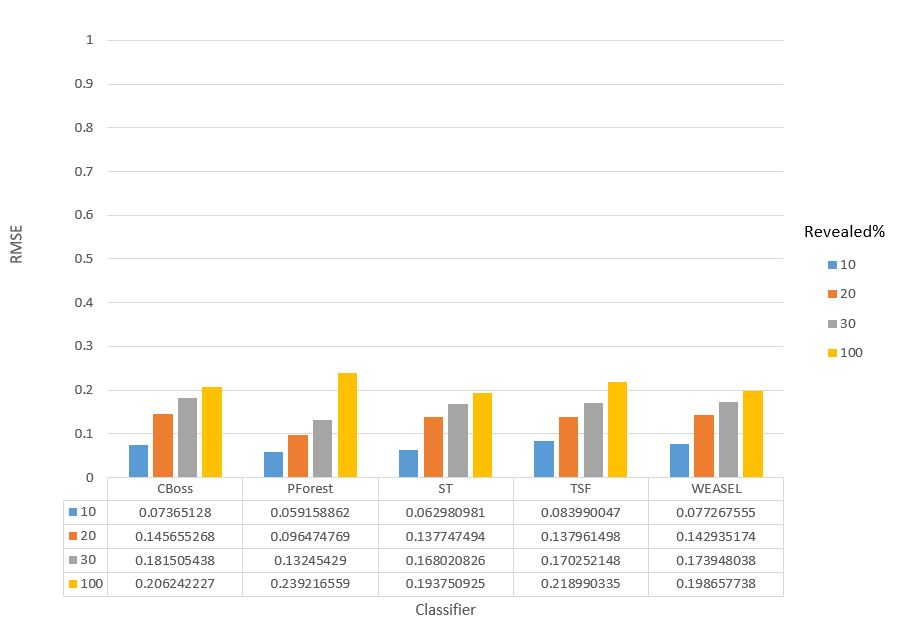
\includegraphics[width=\textwidth]{RMSE_classifier.JPG}
    \centering
    \caption{Avg RMSE for classifiers per chunk over 50 runs}
    \label{Img:RMSEClassifier}
  \end{figure}

\subsection{Which features contribute the most to the F-Score Prediction ?}
\label{SubsectionFeature}
% Feature importance
One of the main reasons why we chose to use random forests for the chunk learners, is that they give a notion of importance for features that were used to build the trees.
This helps understand what features play role in the prediction of scores for the classifiers for each chunk.

Figure \ref{Img:MeanFeatureImportance} shows the average importance of the features across all the 50 runs.
The feature importance is calculated using the default method from the $sklearn$ library; the mean decrease of impurity.
For each selected feature in the internal nodes of the regression trees, the impurity of the split is calculated using variance reduction.
After the whole forest is built, the mean variance reduction for each feature is calculated over all the trees.

\begin{figure}[hp!]
    \captionsetup{justification=raggedright}
    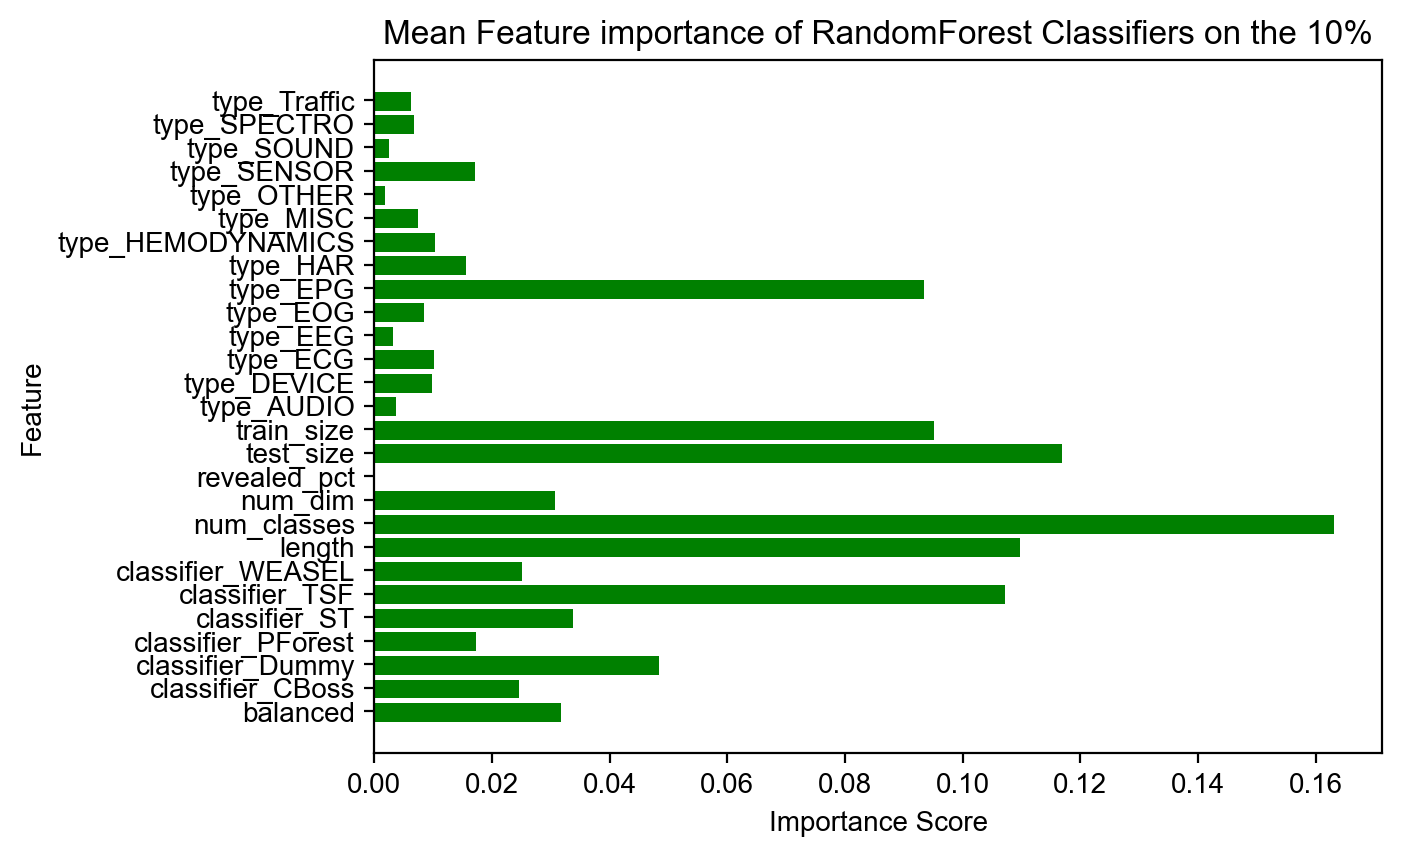
\includegraphics[width=0.49\textwidth,keepaspectratio]{mean_feature_imp_10pct.png}
    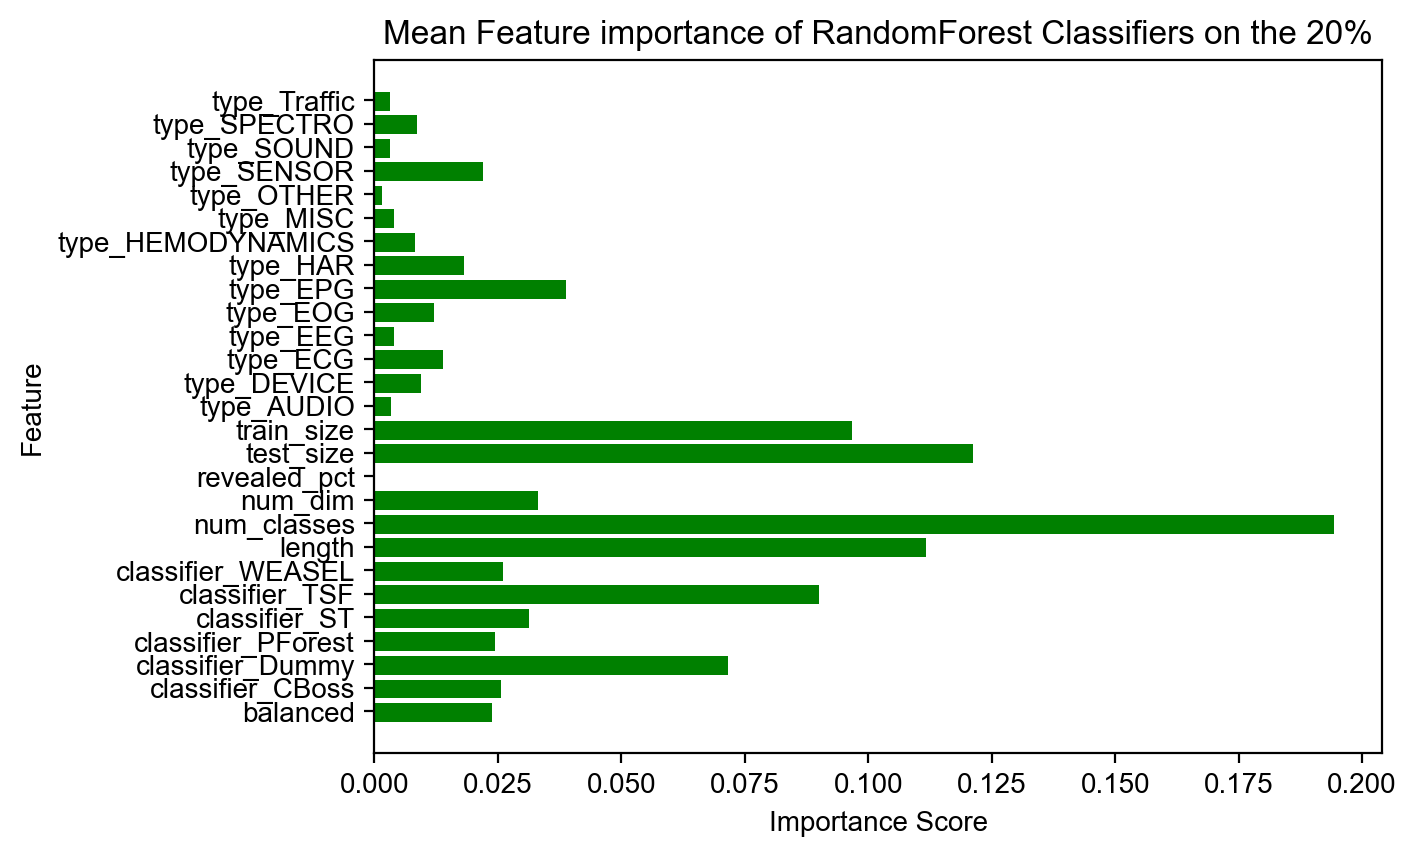
\includegraphics[width=0.49\textwidth,keepaspectratio]{mean_feature_imp_20pct.png}
    \\[\smallskipamount]
    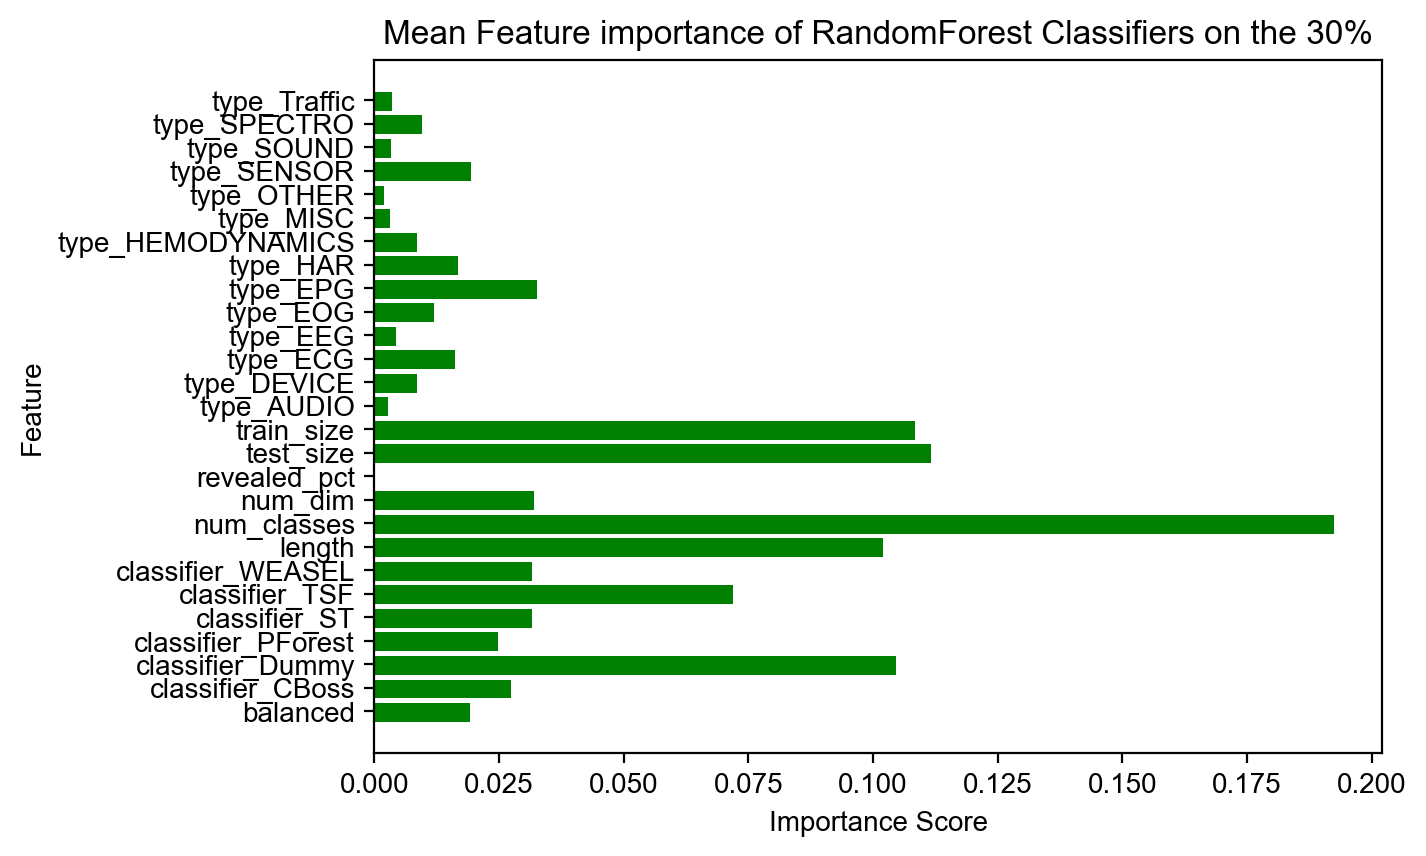
\includegraphics[width=0.49\textwidth,keepaspectratio]{mean_feature_imp_30pct.png}
    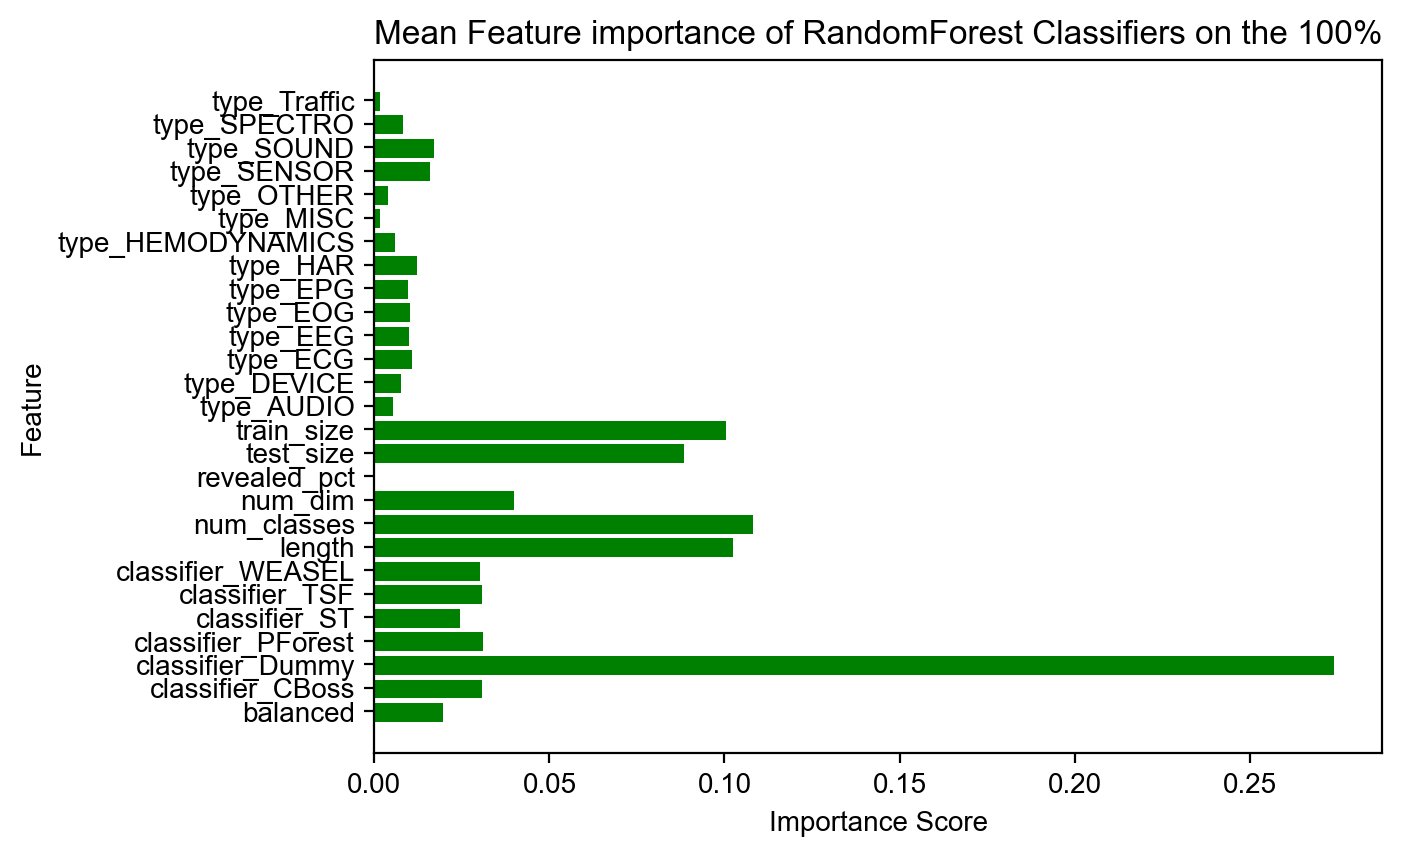
\includegraphics[width=0.49\textwidth,keepaspectratio]{mean_feature_imp_100pct.png}
    \caption{Mean Feature Importance per chunk across 50 runs}
    \label{Img:MeanFeatureImportance}
\end{figure}

For the lower chunk learners, the main metadata of the data sets; number of classes, length, train size and test size have the greatest importances among all the features.
The number of classes persistently has the highest feature importance over all other features.
It is also visible that TSF has high importance on the 10\% chunk results, which conforms with our CD diagram on the 10\% data; due to its significantly better performance.
This importance of TSF fades away as more data is revealed for the classifiers, while on the other hand the imoprtance of the dummy classifier increases.
For the 100\% chunk learner, the Dummy classifier has the highest importance.
This conforms with our results from the CD diagram from Figure \ref{fig:CDAcross},
where all the classifiers are much better than the Dummy classifier; which makes it easy to purely separate from all other results.
This then leads the importance of all the other classifiers to become closer to each other.

\subsection{Are the final recommendations of the framework consistent with actual results ?}
\label{SubsectionFinalRecommendation}
% results for final recommendation
At the end, after all the experiments are finished, the final result of our framework is the suggestions made by the recommender for the user.
For this analysis part, we focus on whether the chunk learners were able to correctly recommend classifiers based on their performance in comparison to the dummy baseline classifier.
A good classifier would be one that can beat the baseline, while a bad classifier is one that doesn't.

% avg accuracy
By aggregating the performance metrics for each chunk learner across the 50 experiments, we can get an overview of their performance.
Table \ref{TableRecommenderOverallPerf} shows the average performance of the 4 chunk learners over all experiments.

\begin{table}[!hbt]
    \centering
    \begin{tabular}{ |c|c|c|c| }
        \hline
        \textbf{Revealed\%} & \textbf{Avg Accuracy} & \textbf{Avg Recall} & \textbf{Avg Precision} \\ \hline
        10 & 73.62 & 0.9520 & 0.6920 \\ \hline
        20 & 80.19 & 0.9597 & 0.7769 \\ \hline
        30 & 86.15 & 0.9925 & 0.8346 \\ \hline
        100 & 95.80 & 0.1000 & 0.9481 \\ \hline
      \end{tabular}
      \caption{Overall Performance of chunk learners in predicting good and bad performers over 50 runs}
      \label{TableRecommenderOverallPerf}
\end{table}

In general, our chunk learners are able to achieve acceptable results in terms of accuracy specially on the full length data.
But accuracy alone is not the best measure to depend on for assessing the results, thus we have a look into the other evaluation metrics.

% insight of the recall
By looking into recall, we score very high results. This means that our chunk learners are able to detect a high majority of the existing good classifiers.
For example, It achieves a recall of 1 on the 100\% data. This indicates that on the full length data, the recommender is able to suggest all the good classifiers.
Although this is a quite impressive result, but we cannot contribute the score to the ability of the classifier to learn on the data.
From our CD diagrams results, we know that the dummy classifier is significantly worse than all the classifiers on the 100\% chunk.
We also know from the F-Score results that the chunk learner on the 100\% data has the highest average RMSE values across all the runs. 
Thus, we believe that the reason such a high score is achieved; is because the dummy classifier is the baseline that decides whether a certain classifier is good or bad.
The dummy classifier is a simple classifier that predicts the majority class and it allows for a wide span of error without affecting the results of the recommendation.
So even if we underestimate the F-scores of the classifiers compared to their actuals, we are still able to get the final suggestions correctly; beause their F-scores are way better than that of the dummy classifier.

% insight of the precision
On the other hand, we can see that our results are not as good when considered from a precision point of view.
This goes back to the nature of the precision measure which focuses on the False Positives in the data.
The same reason that makes the dummy classifier weaker on the full length data, is the one that makes it hard to beat on the shorter length data.
The dummy classifier always predicts the majority class regardless of the length of data.
This means that its balanced accuracy scores are always the same and their total F-scores keep getting better on the lower chunks; because their earliness scores improve as well.
From our CD diagrams results, we know that the dummy classifier is not significantly different than most of the classifiers on the lower chunks.
Thus, the residuals between the actual and predicted F-scores have larger effect and the overestimation of the performance of classifiers is more prominent.

Table \ref{TableClassifierMisestimation} gives a breakdown of the misestimations that the chunk learners did through out the experiments on the classifier level.
From the previous analysis of precision and recall, it is quite obvious that our chunk learners tend to overestimate the performance of the classifiers than to underestimate them.
The misestimation is clearer on the lower chunk predictions, but less obvious on the higher chunks.
This can obviously be recognized in Figure \ref{Img:ActualvsPredScatter} by comparing the vertical distances between the actual and predicted F-scores for each classifier.
TSF is the least misestimated classifier; it is the least overestimated classifier and almost never underestimated.
ST is the second least overestimated classifier, while PForest is the most overestimated.

\begin{figure}[hp!]
    \captionsetup{justification=raggedright}
    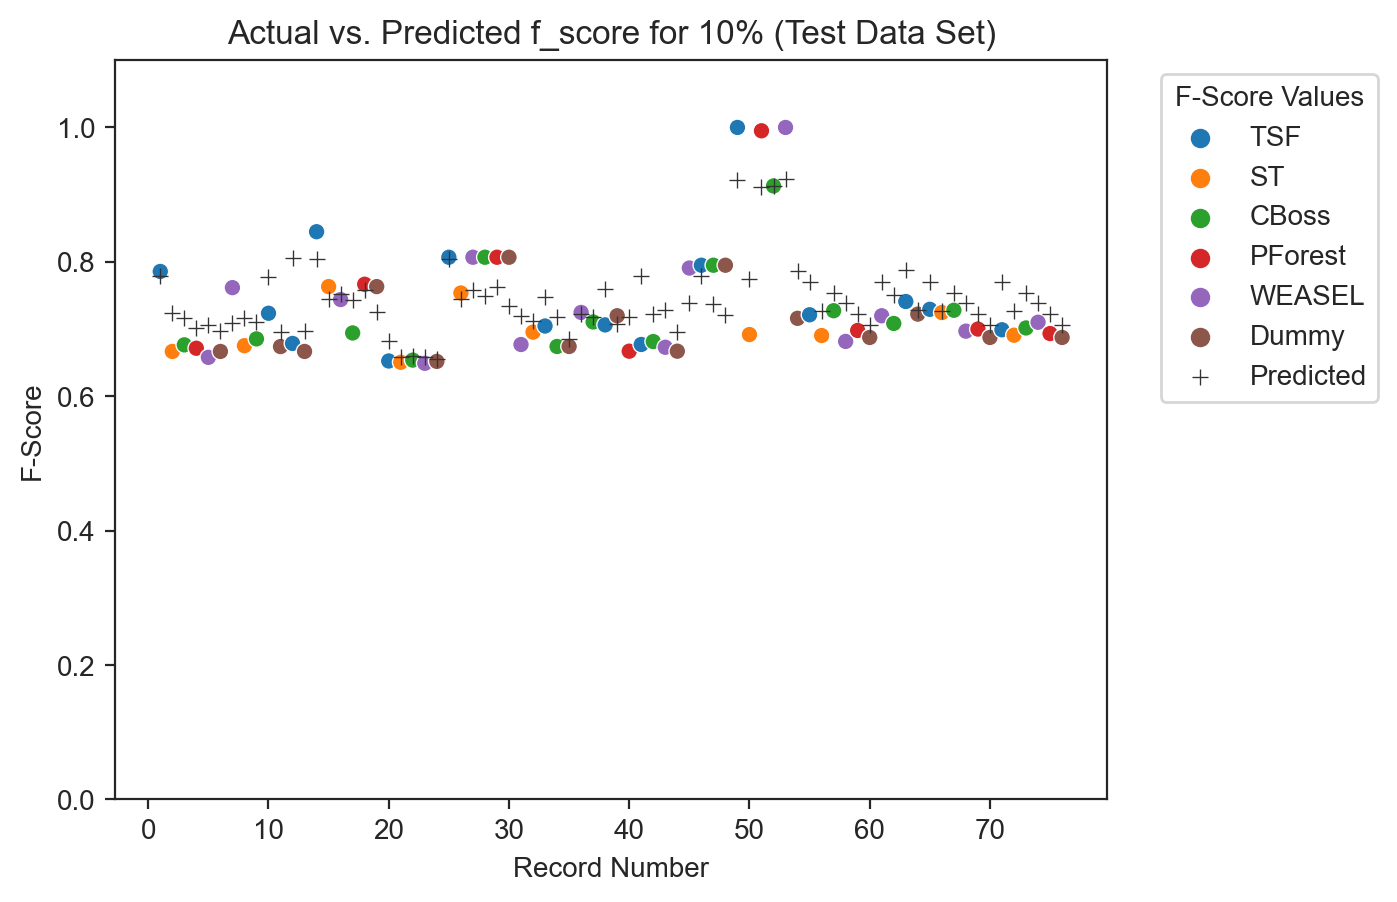
\includegraphics[width=0.49\textwidth,keepaspectratio]{scatter_test_actual_vs_pred_10pct.png}
    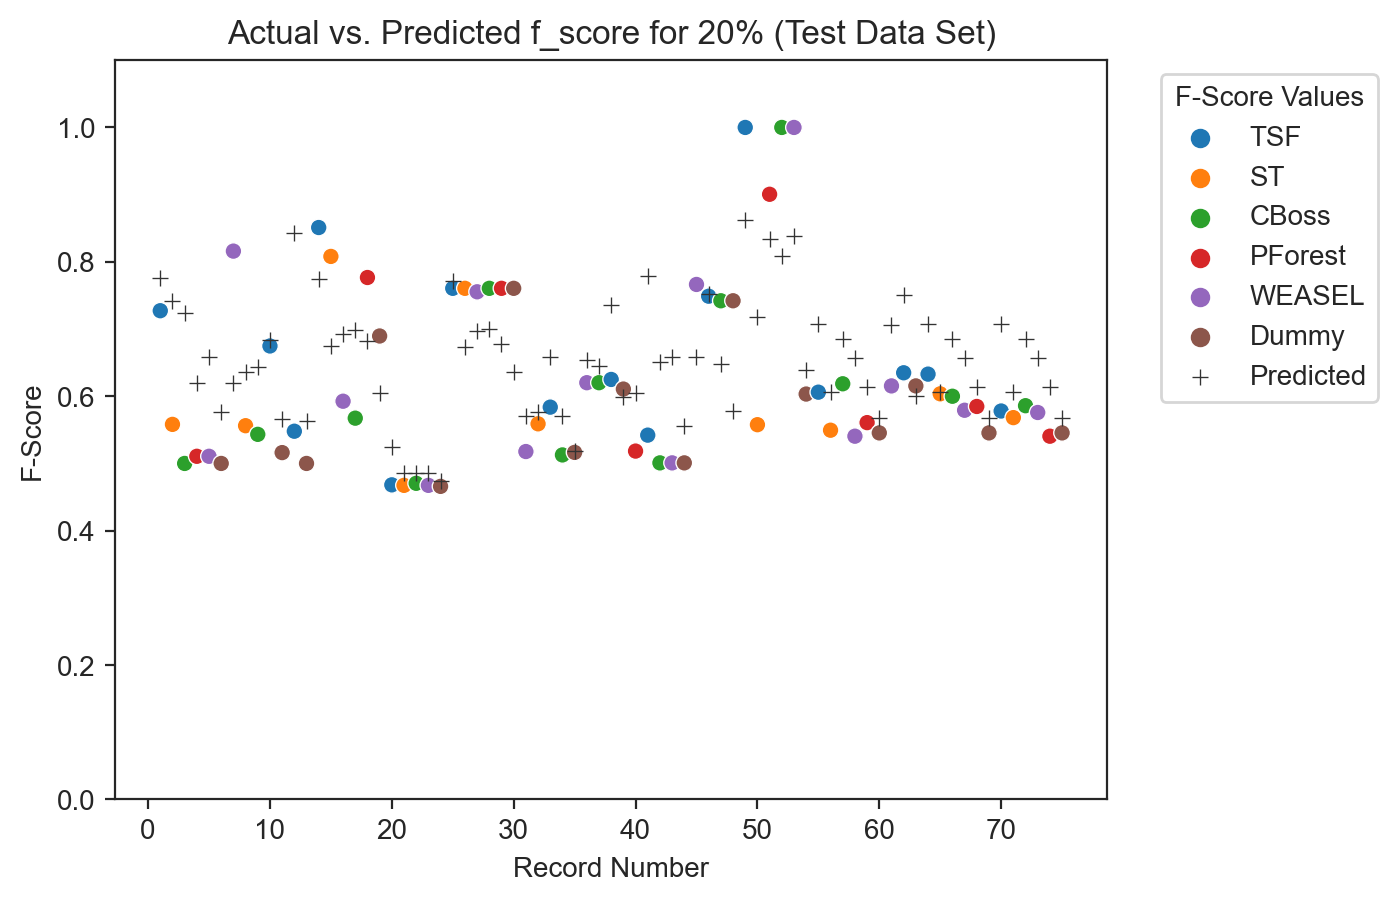
\includegraphics[width=0.49\textwidth,keepaspectratio]{scatter_test_actual_vs_pred_20pct.png}
    \\[\smallskipamount]
    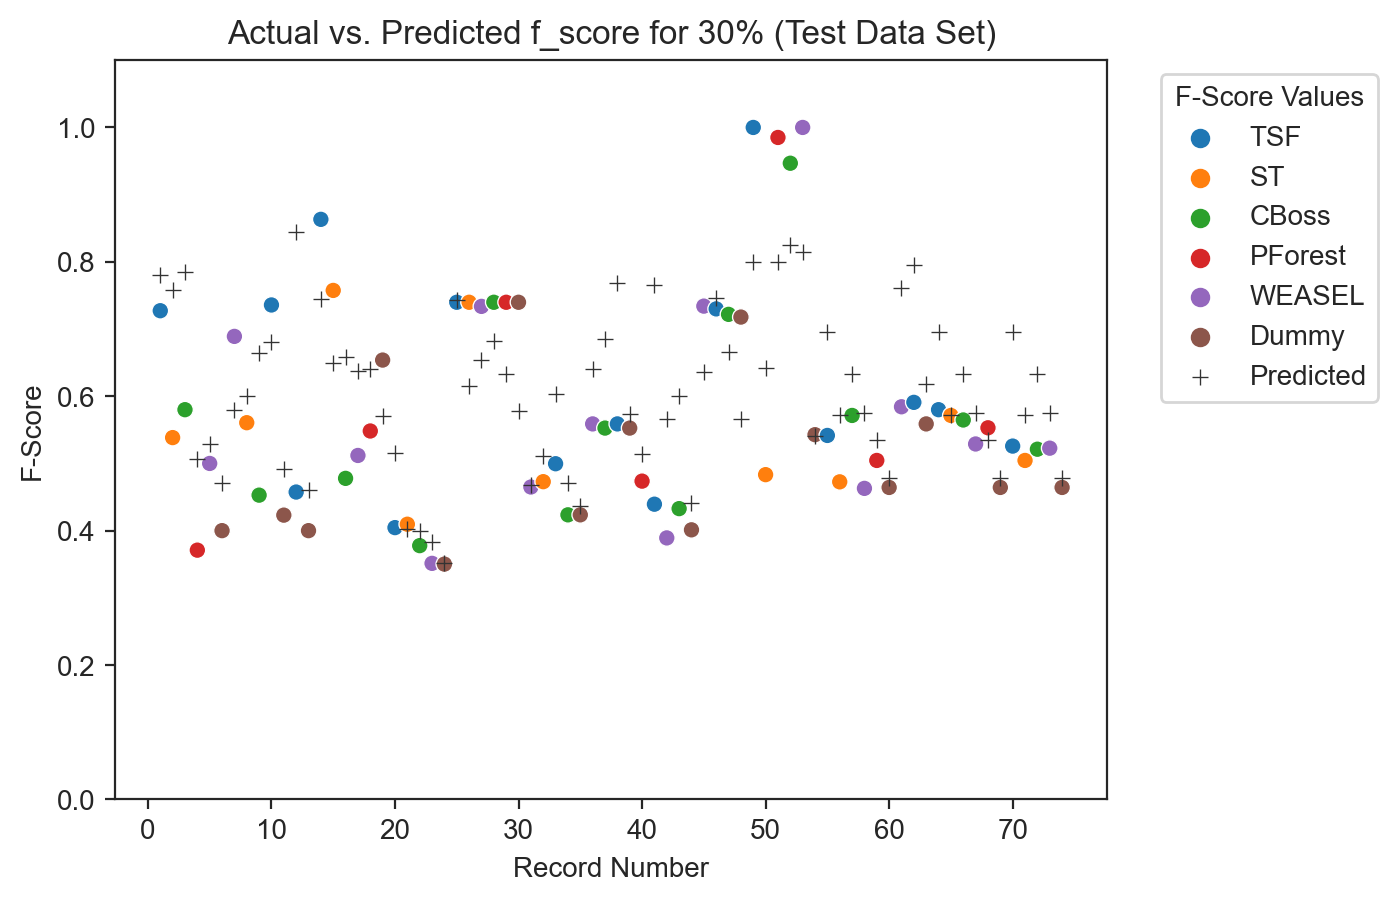
\includegraphics[width=0.49\textwidth,keepaspectratio]{scatter_test_actual_vs_pred_30pct.png}
    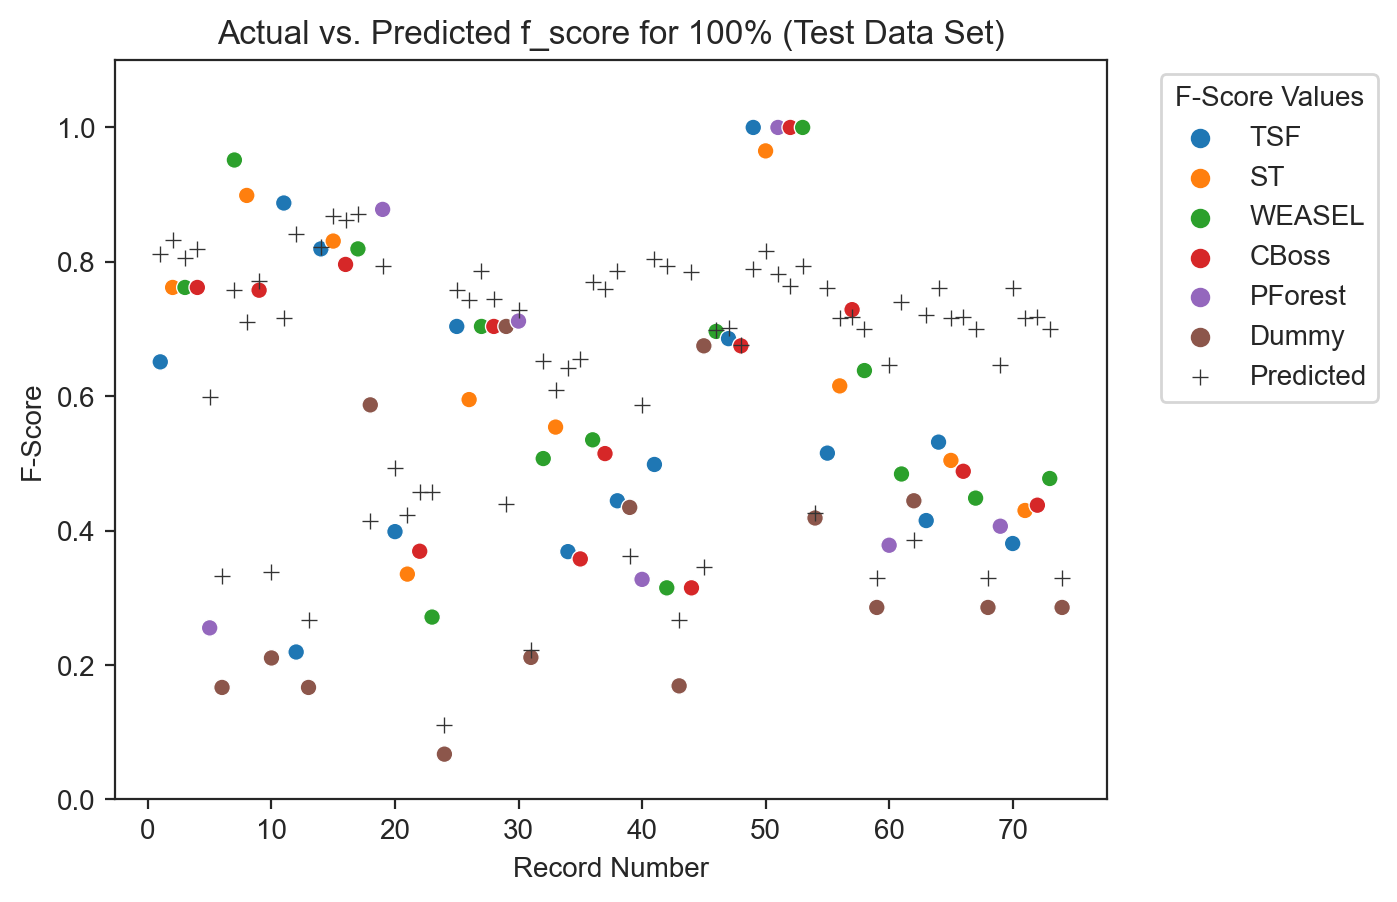
\includegraphics[width=0.49\textwidth,keepaspectratio]{scatter_test_actual_vs_pred_100pct.png}
    \caption{Actual vs. Predicted F-score for chunk learners (experiment seed = 22)}
    \label{Img:ActualvsPredScatter}
\end{figure}

\begin{landscape}
  \begin{table}[hp!]
    \setlength\extrarowheight{2pt} % for a bit of visual "breathing space"
    \begin{tabularx}{\hsize}{|X|X|X|X|X|X|X|X|X|}
    \hline
    %\textbf{Classifier} & \textbf{Revealed\%} & \textbf{Total Tests} & \textbf{\#Overestimate} & \textbf{\#Underestimate}  & \textbf{Overestimate\%} & \textbf{Underestimate\%} & \textbf{\#Misestimation} & \textbf{Misestimation\%} \\ \hline
    \textbf{Classifier} & 
    \textbf{Revealed} & 
    \textbf{Total} & 
    \textbf{\#Overest-} & 
    \textbf{\#Underest-}  & 
    \textbf{Overest-} & 
    \textbf{Underest-} & 
    \textbf{\#Misest-} & 
    \textbf{Misest-} \\
    &
    \textbf{\%} & 
    \textbf{Tests} & 
    \textbf{imations} & 
    \textbf{imations}  & 
    \textbf{imations\%} & 
    \textbf{imations\%} & 
    \textbf{imations}  & 
    \textbf{imations\%}\\
    \hline
    CBoss   & 10 & 726 & 226 & 36 & 31.13\% & 4.96\% & 262 & 36.09\% \\ \hline
    CBoss   & 20 & 717 & 204 & 20 & 28.45\% & 2.79\% & 224 & 31.24\% \\ \hline
    CBoss   & 30 & 717 & 108 & 2 & 15.06\% & 0.28\% & 110 & 15.34\% \\ \hline
    CBoss   & 100 & 717 & 46 & 0 & 6.42\% & 0.00\% & 46 & 6.42\% \\ \hline
    PForest & 10 & 477 & 204 & 16 & 42.77\% & 3.35\% & 220 & 46.12\% \\ \hline
    PForest & 20 & 477 & 104 & 24 & 21.80\% & 5.03\% & 128 & 26.83\% \\ \hline
    PForest & 30 & 454 & 154 & 5 & 33.92\% & 1.10\% & 159 & 35.02\% \\ \hline
    PForest & 100 & 417 & 32 & 0 & 7.67\% & 0.00\% & 32 & 7.67\% \\ \hline
    ST      & 10 & 618 & 165 & 31 & 26.70\% & 5.02\% & 196 & 31.72\% \\ \hline
    ST      & 20 & 618 & 155 & 26 & 25.08\% & 4.21\% & 181 & 29.29\% \\ \hline
    ST      & 30 & 618 & 78 & 3 & 12.62\% & 0.49\% & 81 & 13.11\% \\ \hline
    ST      & 100 & 618 & 19 & 0 & 3.07\% & 0.00\% & 19 & 3.07\% \\ \hline
    TSF     & 10 & 745 & 74 & 4 & 9.93\% & 0.54\% & 78 & 10.47\% \\ \hline
    TSF     & 20 & 745 & 46 & 2 & 6.17\% & 0.27\% & 48 & 6.44\% \\ \hline
    TSF     & 30 & 745 & 26 & 1 & 3.49\% & 0.13\% & 27 & 3.62\% \\ \hline
    TSF     & 100 & 745 & 35 & 0 & 4.70\% & 0.00\% & 35 & 4.70\% \\ \hline
    WEASEL  & 10 & 731 & 277 & 31 & 37.89\% & 4.24\% & 308 & 42.13\% \\ \hline
    WEASEL  & 20 & 731 & 193 & 25 & 26.40\% & 3.42\% & 218 & 29.82\% \\ \hline
    WEASEL  & 30 & 731 & 169 & 10 & 23.12\% & 1.37\% & 179 & 24.49\% \\ \hline
    WEASEL  & 100 & 726 & 34 & 0 & 4.68\% & 0.00\% & 34 & 4.68\% \\ \hline
    \caption{Misestimation results per classifier per chunk learner over 50 runs}
    \label{TableClassifierMisestimation}
  \end{tabularx}
  \end{table}
\end{landscape}